\documentclass[a4paper,10pt]{report}

\usepackage[utf8]{inputenc}
%\usepackage[T1]{fontenc}
%\usepackage[french]{babel}
\usepackage[margin=1in]{geometry} 
\usepackage{amsmath,amsthm,amssymb}
\usepackage{algorithm}
\usepackage{algorithmic}
\usepackage{lmodern}
\usepackage{graphicx}
\usepackage{mathtools}
\usepackage{tcolorbox}
\usepackage{listings}
\usepackage{subcaption} % pour le subplot
\usepackage{fancyhdr}
\usepackage[bottom]{footmisc}
\usepackage[hidelinks]{hyperref}
\usepackage{xcolor}
\usepackage[framemethod=tikz]{mdframed}
\usepackage{varwidth}
                                                                       
% Specific font for headings 


\pagestyle{fancy}
\newcommand{\R}{\mathbb{R}}  
\newcommand{\Z}{\mathbb{Z}}
\newcommand{\N}{\mathbb{N}}
\newcommand{\Q}{\mathbb{Q}}
\newcommand{\C}{\mathbb{C}}
\DeclareMathOperator*{\argmax}{arg\,max}
\DeclareMathOperator*{\argmin}{arg\,min}


%opening
\title{Intership - Sparse Coding and Dictionary learning}
\author{Thomas Rolland}
\date{}%Remove date

\begin{document}


\begin{titlepage} % Suppresses displaying the page number on the title page and the subsequent page counts as page 1
	\newcommand{\HRule}{\rule{\linewidth}{0.5mm}} % Defines a new command for horizontal lines, change thickness here
		%------------------------------------------------
	%	Logo
	%------------------------------------------------
	
	
\includegraphics[scale=0.2]{siteon0.png} % Include a department/university logo - this will require the graphicx package
\hfill
 \includegraphics[scale=2]{SAMoVA.png}
 % SAMoVA.png: 226x110 px, 300dpi, 1.91x0.93 cm, bb=0 0 54 26

	\center % Centre everything on the page
	
	%------------------------------------------------
	%	Headings
	%------------------------------------------------
	
	\textsc{\Large Final Graduation Project Report}\\[1.5cm] % Main heading such as the name of your university/college
	
	\textsc{\Large Institut de Recherche en Informatique de Toulouse - IRIT}\\[0.5cm] % Major heading such as course name
	
	\textsc{\large SAMoVA}\\[0.5cm] % Minor heading such as course title
	
	%------------------------------------------------
	%	Title
	%------------------------------------------------
	
	\HRule\\[0.4cm]
	
	{\huge\bfseries Statistical methods vs. Neural network 
\\ \vspace{0.5cm}- \vspace{0.5cm} \\  Comparison of methods for learning units using Dictionary Learning and Sparse Coding vs Auto-encoders}\\[0.4cm] % Title of your document
	
	\HRule\\[1.5cm]
	
	%------------------------------------------------
	%	Author(s)
	%------------------------------------------------
	
	\begin{minipage}{0.4\textwidth}
		\begin{flushleft}
			\large
			\textit{Author}\\
			Thomas \textsc{Rolland} % Your name
		\end{flushleft}
	\end{minipage}
	~
	\begin{minipage}{0.4\textwidth}
		\begin{flushright}
			\large
			\textit{Supervisors}\\
			Thomas \textsc{Pellegrini}\\ % Supervisor's name\\
			Adrian \textsc{Basarab}\\ \vspace{0.2cm}
            Carine \textsc{Jauberthie}
            
		\end{flushright}
	\end{minipage}
	
	% If you don't want a supervisor, uncomment the two lines below and comment the code above
	%{\large\textit{Author}}\\
	%John \textsc{Smith} % Your name
% 	
	%------------------------------------------------
	%	Date
	%------------------------------------------------
	
	\vfill
	\begin{center}
 
\includegraphics[scale=1]{Logo_UT3.jpg}
 % Logo_UT3.jpg: 799x269 px, 300dpi, 6.76x2.28 cm, bb=0 0 192 65
\end{center}

	\vfill % Position the date 3/4 down the remaining page
	
	{\large\today} % Date, change the \today to a set date if you want to be precise
	

	%----------------------------------------------------------------------------------------
	
	\vfill % Push the date up 1/4 of the remaining page
	
\end{titlepage}

% \begin{abstract}
% Nowadays deep learning methods allow to have state-of-the-art results for many tasks. Here we focus on discriminant parameter extraction using statistical and deep learning methods. Our objective was to compare different methods to know which of these two approaches is useful in our problem. It has been shown that deep learning allows better results than statistical approaches. In addition, we have proposed a new autoencoder model that uses an idea from the statistical approach. This new autoencoder is the best method we've used to solve this problem.\\
% \end{abstract}

\chapter*{Remerciements}

Je voudrais remercier toute l'équipe SAMoVA sans laquelle ce stage n'aurait jamais eu lieu. Merci de leurs accueils ainsi que leurs précieux conseils pendant ces cinq mois. Je souhaiterais notamment remercier Thomas Pellegrini d'avoir encadré ce stage, pour ses conseils, ses idées, sa patience et son accueil. Il mérite amplement son nom de Monsieur "Deep Learning" de SAMoVA.\\

Je voudrais aussi remercier Adrian Basarab d'être intervenu comme expert des méthodes de Sparse Coding, ses conseils ont été précieux dans la réussite de ce stage.\\

Ce stage n'aurait pas été ce qu'il a été sans la présence des différents doctorants et stagiaires des différentes équipes du Thème 1. Merci à eux de m'avoir permis de travailler dans une bonne ambiance.\\

Je souhaiterais naturellement remercier aussi mes proches, ma famille, mes amis.\\

Certain d'oublier quelqu'un, je remercie aussi tous ceux qui ont participés à ce stage, de près ou de loin.\\

\vspace{10cm}\hspace{7cm} J'ai aussi une pensée pour Mamie Brest et Lili.
\newpage
\tableofcontents

\chapter{Introduction}


\label{chap:Introduction}
\section{Hosting Laboratory}
In the context of my master's degree, I did 5 months of internship in the SaMova team in IRIT laboratory.\\

The IRIT (\textbf{I}nstitut de \textbf{R}echerche en \textbf{I}nformatique de \textbf{T}oulouse – \textbf{I}nformatics \textbf{R}esearch \textbf{I}nstitute of \textbf{T}oulouse) represents one of the major laboratories of the French research in computer science, with a workforce of more than 700 members including 272 researchers and teachers 204 PhD students, 50 post-doc and researchers under contract and also 32 engineers and administrative employees.\\
The 21 research groups of the laboratory are dispatched in seven scientific themes covering all the computer science domains of today :
\begin{itemize}
 \item 1 : Information Analysis and Synthesis
 \item 2 : Indexing and Information Search
 \item 3 : Interaction, Autonomy, Dialogue and Cooperation
 \item 4 : Reasoning and Decision
 \item 5 : Modelization, Algorithms and High-Performance Calculus
 \item 6 : Architecture, Systems and Networks
 \item 7 : Safety of Software Development
 
\end{itemize}

SAMoVA (\textbf{S}tructuration, \textbf{A}nalysis, \textbf{Mo}delling of \textbf{V}ideo and \textbf{A}udio documents) team, include into the Topic 1 - Information Analysis and Synthesis, focuses its research activities mainly on audiovisual contents. Those works are applied on different kinds of content such as audiovisual content analysis, spoken content analysis, analysis of pathological voice, ...\\

\section{Context}

Since time immemorial, speech has been the most important means of communication among humans. By definition, speech is the ability or act of expressing or describing thoughts, feelings or perceptions through the articulation of words. To do this, humans use their vocal apparatus (lungs, glottis, larynx, tongues, lips, jaws, \dots) to produce "syllables" that fuse to form words and phrases. \newline

Speech recognition allows the captured human voice to be analyzed and transcribed into machine-readable text. Over the past decades, automated speech recognition has become one of the major fields of artificial intelligence and signal processing. Indeed, since the introduction to our daily lives of artificial personal assistants like Siri or Google Assistant, speech recognition systems must answer more complex demands. To achieve this level of complex problem solving, these systems must first understand what the user has said, i.e. do good speech recognition. \newline

Recently, the speech recognition field has benefited from advances in deep learning with neural network methods to improve results and advanced technologies.\\
Speech recognition is traditionally based on two steps (see figure \ref{fig: Speech Procesing expain}):\\
\begin{itemize}
 \item 
First, the raw signal is transformed by a feature extractor to give a new representation of this signal, with more relevant information (generally we use Mel Frequency Cepstral Coefficients as a new representation for speech processing).
\item 
 Second, for speech recognition, this new representation is given as the input of a classifier that will give us the text translation of our input signal.

\end{itemize}
\begin{figure}[h]
 \hspace{-1cm}
 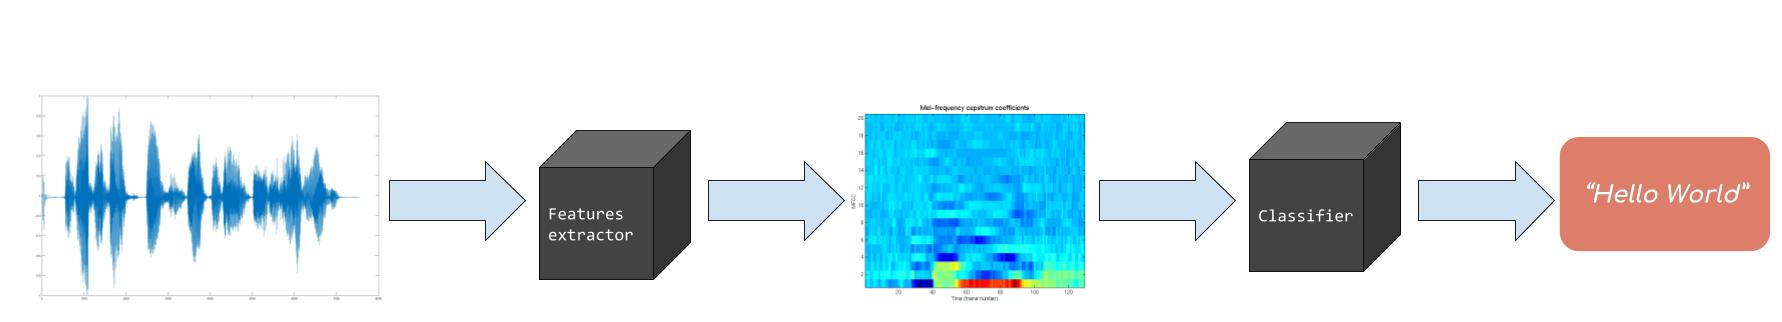
\includegraphics[scale=0.27]{Speech_Processing.jpg}
 % Speech Processing.jpg: 1782x322 px, 72dpi, 62.87x11.36 cm, bb=0 0 1782 322
 \caption{Basic pipeline of speech recognition}
 \label{fig: Speech Procesing expain}
\end{figure}
The goal of my internship is to find a new kind of feature extractor using deep learning and statistical methods. Compare the discriminating power of each of them for signal processing in a generic approach, whether we work on images or sounds. Our work was mainly focused on images using the MNIST dataset since working on the sound level is similar. Indeed the sound signal is transformed into a spectrogram like that will be used as an image to feed the models.

%In order to focus later on only one type of signal: Speech, because work on the spectrograms of the speech signal is the same as work on an image. This is why during this internship we decide to limit our work to the MNIST dataset, a widely used dataset.\\

The chosen methods to replace the traditional feature extractor are:
\begin{itemize}
 \item Auto-Encoder as a Deep learning approach
\item  Sparse Coding a Statistical approach
\end{itemize}
However, the main focus of this internship has been on the statistical methods due to the recent interest of the signal processing community in this kind of method.
\section{Organization}
The present report is organized as follows:
\begin{itemize}
 \item  \textbf{Chapter \ref{chap:SparseCoding}}:  Explain the principle of traditional Sparse Coding, how it is done and give an example on MNIST dataset.
 \item \textbf{Chapter \ref{chap:Discriminative}}: Show the problem with traditional Sparse coding for classification and bring a new solution to obtain a discriminative Sparse code for classification.
 \item \textbf{Chapter \ref{chap:Conv}}: Here, we will explain the natural extension of traditional Sparse Coding to handle shift-variance.
 \item \textbf{Chapter \ref{chap:SupervisedConv}}: As we did in chapter \ref{chap:Discriminative} for traditional Sparse coding, we will explain one method to obtaining discriminatory Sparse coding in Convolution Sparse Coding.
 \item \textbf{Chapter \ref{chap:AE}}: We present the deep learning methods with which we compare Sparse Coding.
 \item \textbf{Chapter \ref{chap:Conclusion}}: Explain our results and the different perspectives we have.
\end{itemize}


\newpage
\chapter{Traditional Sparse Coding}
\label{chap:SparseCoding}
%\documentclass[SparseCoding.tex]{subfiles}
\section{\textit{Sparseland}}

Modeling data play a central role in signal processing and machine learning. Sparse representation model also refers as \textit{Sparseland} \cite{8398588},  suggests a description of every signal as sparse linear combinations of basic elements called \textit{atoms}, which come from a redundant matrix called a \textit{dictionary}. Redundant matrix means that we have more atoms than the size of the corresponding signal. \\
The Sparseland model became one of the most important modelizations in image processing, and more generally in signal processing. Its give state-of-the-art results in a wide variety of tasks: Denoising, inpainting, image separation, deblurring,\dots\\
There is one fundamental property on which this theory is based, the same property which allows us to compress a signal, to denoise, enhance a degraded signal, \dots. All meaningful data sources (i.e signal) are structured.\\
Each source of information: image, audio, video, 3D object (meshes or points cloud),  text, financial time series, data on a graph,\dots  have an inner structure that is unique to them which can be characterized in various ways and allow redundancy.\\

The first signs of \textit{Sparseland} appear in the 1990s with the greedy and relaxed pursuit algorithm \cite{258082,305222} and the introduction of dictionary learning \cite{Olshausen97sparsecoding}.

\subsection*{The idea behind \textit{Sparseland}}
The first step in \textit{Sparseland} is to find (i.e learn) a dictionary with a relevant set of atoms (this step is called \textbf{Dictionary Learning}). Then the model assumption is that every incoming signal could be represented as a linear combination of only a few atoms from the dictionary (this step is called \textbf{Sparse Coding}).\\ \vspace{-0.4cm}
\begin{center}
\fbox{\begin{varwidth}{\textwidth}
\centering
\hspace{-5.5cm}\textbf{Definition:} Sparse \\ \vspace{0.2cm} \textit{ Occurring at widely spaced intervals, not thick or dense.}
\end{varwidth}}
%\fbox{\textbf{Definition:} \\Sparse:
%\textit{ Occurring at widely spaced intervals, not thick or dense.}}
\end{center}\vspace{0.4cm}
Unlike decomposition based on principal component analysis, \textit{Sparseland} does not impose that learned representation to be orthogonal, allowing more flexibility to adapt the representation to the signal.
\\
The idea of finding new representations of an input signal is not new. Signal processing's scientists already use this approach with predefined dictionaries instead of a learned one, for example, wavelets transform or Fourier transform. With a learned dictionary, we can expect to get more relevant information about the inner structure of the signal. For that reason, we can expect better performances in a wide range of applications.

\section{Mathematical formulation}


 \begin{figure}[h]
 \centering
 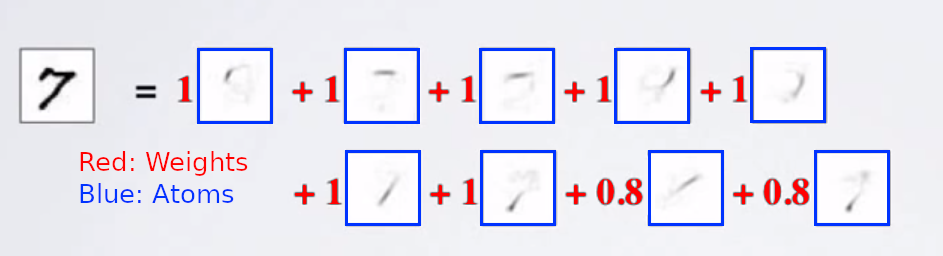
\includegraphics[scale=0.5]{spacecoding_12.png}
 % spacecoding_1.png: 943x256 px, 96dpi, 24.95x6.77 cm, bb=0 0 707 192
 \caption{Example of Sparse Coding reconstruction}
 \label{fig:exemple}
\end{figure}

Consider a signal $x_i \in \R^m$ in a set of signal $X = [x_1, x_2, \ldots, x_n] \in \R^{m \times n}$ ( generally $n$ is large and $m$ is small: $n >> m$), the aim of this method is to find a linear combination of overcomplete basis elements $D = [d_1, d_2, \ldots, d_k]$ under sparsity constraints which reconstruct the input signal (see  an example at figure \ref{fig:exemple}), overcomplete dictionary mean that $k > m$:
\begin{center}
 $x_i = D \gamma_i$
 \\ With $\gamma_i$ the sparse coefficients of the sparse decomposition for the signal $x_i$
\end{center}

The traditional way to get $\gamma_i$ is to optimize the empirical cost function.
\begin{center}
 $f_n(D) = \frac{1}{n} \sum_{i=1}^{n} l (x_i,D)$
\end{center}
Where $l$ is the cost function which is small where D is good for representing the signal. Usually, we use :
\begin{center}
 $l(x_i,D) =   \min\limits_{\gamma_i} \frac{1}{2} \underset{Squared\ error}{\underbrace{\| x_i - D \hspace{3px} \gamma_i \|_2^2}} + \lambda \underset{Sparsity\ term}{\underbrace{ \|\gamma_i \|_0}}$
\end{center}
Note that the cost function has two terms, which fight each other.  The first term corresponds to the squared error, while that the second term corresponding to the sparsity of the weight vector. $\lambda$ is a positive constant which controls the importance of the sparse term relative to the square error term. \\
The norm of all columns of D must be equal or less than 1  , otherwise, D could grow big while $\gamma$ becomes small to satisfy the prior.\\
This problem is also known as a \textit{basic pursuit}  or the  \textit{Lasso}. However, it is important to notice that the problem isn't convex and his optimization is NP-complete (due to the $l_0$ norm). Fortunately, it is well known that for kind of problem use $l_1$ norm instead of $l_0$ norm yields a sparse solution for $\gamma_i$.\\
Then the optimization problem can be rewritten as:
\begin{center}
 $\min\limits_{D} \frac{1}{n} \sum_{i=1}^{n}  \min\limits_{\gamma_i} \frac{1}{2} \| x_i - D \hspace{3px} \gamma_i \|_2^2 + \lambda \|\gamma_i \|_1$
\end{center}
Before presenting our experimentations we will explain how traditional Sparse Coding works. In particular, how this method learns redundant properties and patterns in a signal set. This is the learning phase.
\newpage
\section{Learning step}
A natural approach to solve this optimization problem is to alternate between the optimization of $D$ and $\gamma$, minimize over one while keeping the other one fixed.\\
\begin{algorithm}
 \label{algo:algo1}

 \caption{Learning step}
 \begin{algorithmic}
 \REQUIRE X the input signal
    \STATE $D_0$ initilized randomly, $\gamma$  is a zeros matrix
    \WHILE{D and $\gamma$ not converged}
        \STATE Fix D
        \STATE Find $\gamma$ \hspace{0.7cm} \textit{/* Sparse Coding step */}   (1)
        \STATE Fix $\gamma$
        \STATE Find D \hspace{0.7cm} \textit{/*Dictionary Learning  */} (2)
    \ENDWHILE
 \end{algorithmic}

\end{algorithm}

% 
% \paragraph{Idea} Sparse dictionary learning is a representation learning method which aims at finding a sparse representation of the input data (in form of a linear combination of basic elements (called Atoms). The idea of using a learned dictionary instead of a predefined one is based on wavelets.  The sparse learned models has recently led to state-of-the-art result for denoising, classification,...
% %UNSPERVISED LEARNING=========================================================+
% \paragraph{Unsupervised learning} Only use the inputs $x^{(t)}$ ( $X = [x_1,....,x_n]$ in $\R^{m \times n}$) for learning. Automatically extract meaningful features of our data, leverage the availability of unlabeled data and add a data-dependent regularize to trainings.\\
% 
% Sparse coding is one of the methods used for unsupervised learning  (like restricted Boltzmann machines and autoencoders).\\
% The idea behind sparse coding is: For each $x^{t}$ find a latent representation $\gamma^{t}$ such that:
% \begin{itemize}
%  \item[$\bullet$] It is sparse: the vector $\gamma^{t}$ has many zeros (only few nonzero elements)
%  \item[$\bullet$] We can reconstruct the original input $x^{(t)}$ as well as possible.
% \end{itemize}
% That mean, more formally:\\
% 
% %Formulation du problème=============================
% \begin{center}
%  $\min\limits_{D} \frac{1}{T} \sum_{t=1}^{T}  \min\limits_{\gamma^{(t)}} \frac{1}{2} \| x^{(t)} - D \hspace{3px} \gamma^{(t)} \|_2^2 + \lambda \|\gamma^{(t)} \|_1$\\
% \end{center}
% 
%  %Explicaiton de la formulation=========================
%  \begin{itemize}
%  \item[$\bullet$] D is a matrix of weights, usually refer to that matrix as a dictionary matrix (containt atoms) with $D \in  \R^{m \times k}$ ( k the number of atoms)
%   \item[$\bullet$] $\| x^{(t)} - D \hspace{3px} \gamma^{(t)} \|_2^2 $ is the reconstruction error
%   \item[$\bullet$]$ D \hspace{3px} \gamma^{(t)}$ is the reconstruction of $\hat{x}^{(t)}$
%   \item[$\bullet$]$\|\gamma^{(t)} \|_1$ is the sparsity penalty (more 0 in h we have, better it is)
%  \end{itemize}
% This two objectives fight each other. But it still a optimization problem (cf min), and we'll try to optimize it for each training example $x^{(t)}$. This is why we have a sum over all the training examples.
% \newline
% 
% %Contraintes sur D======================================
% \indent We also constrain the columns of D to be of norm 1 (otherwise, D could grow big while $\gamma^{(t)}$ becomes small to satisfy the prior). And sometimes the columns are constrained to be no greather than 1.\\
% 
% However, $\gamma^{(t)}$ is now a complicated function of $x^{(t)}$:\\
% Encoder is the minimization $\gamma(x^{(t)}) = arg\min\limits_{\gamma^{(t)}}= \frac{1}{2} \| x^{(t)} - D \hspace{3px} \gamma^{(t)} \|_2^2 + \lambda \|\gamma^{(t)} \|_1$, so the optimization problem is more complicated than a simple non linear problem.\\
% The idea to solve this minimization problem is \cite{NIPS2006_2979}
% 
% \begin{lstlisting}[language=Python,frame=single]
% while D not_converged :
%     Fix D
%     Minimize alpha     (1) // Sparse Coding step
%     Fix alpha
%     Minimize D           (2) // Update Dictionary step
% \end{lstlisting}
% 
% But there are some improvement like K-SVD algorithm \cite{KSVD}, which compute column by column a SVD computation over the relevant examples.
% %DICTIONARY==================================================================+  
% \paragraph{Dictionary}
% We can also write $\hat{x}^{(t)} = D\hspace{3px} \gamma(x^{(t)}) \displaystyle\sum_{\substack{k s.t.\\ \gamma(x^{(t)})_k\neq 0}}  D.,_k \gamma(x^{(t)} )_k$
% \begin{figure}[h]
%  \centering
%  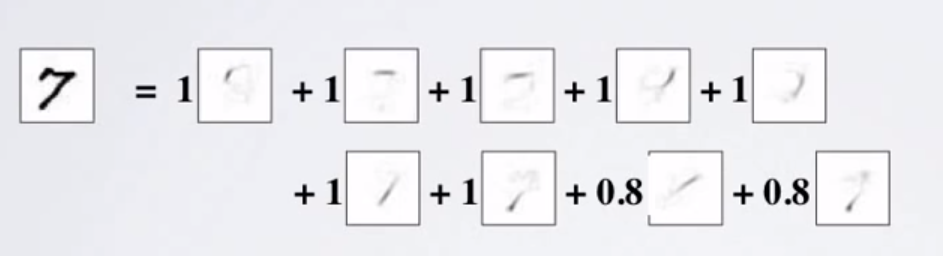
\includegraphics[scale=0.5]{spacecoding_1.png}
%  % spacecoding_1.png: 943x256 px, 96dpi, 24.95x6.77 cm, bb=0 0 707 192
%   \caption{Example of reconstruction using sparse coding}
% \end{figure}
% 
% The images refer to $D.,_k$ (columns of D wich are not equals to 0) and the factor (1 or 0.8 in this case) refer to $\gamma(x^{(t)} )_k$
% \\We also refer to D as the dictionary:
% \begin{itemize}
%  \item[$\bullet$]in certain applications, we know what dictionary matrix to use
%  \item[$\bullet$]often however, we have to learn it
% \end{itemize}
% 
% In general we have $k<<n$ . But we can use an overcomplete dictionary with $k > m$.
% 
%\end{document}

\subsection{Inference of Sparse code}
The original problem is a combinatorial problem (proven to be NP-hard). To solve this problem we use relaxation methods (then we can smooth the $L_0$ and use continuous optimization techniques) or greedy methods (then build the solution one non-zero element at time).
\subsubsection{Compute $\alpha$ }
%Inderence of sparse code=============================================
\paragraph{Idea}
Here we develop  step (1) of our algorithm.\\
Assume we are given a dictionary matrix D, how do we compute $h(x^{(t)})$. We have to optimize:
\begin{center}  Basic Pursuit:
$l(x^{(t)}) = \frac{1}{2} \| x^{t}- D \alpha^{(t)} \|^{2}_{2} + \lambda \|\alpha^{(t)}\|_1 w.r.t. \alpha^{(t)}$\\ 
\end{center} 
Here we used relaxation method to switch from norm $l_0$ to $l_1$ know as the  Basic Pursuit (vs Matching Pursuit, a greedy method,  if we keep $l_0$ norm and find one atom at a time).\\
We could use a gradient descent method to solve this minimization:\\
\begin{center}
$\Delta_{\alpha^{(t)}} l(x^{(t)}) = D^T (D \alpha^{(t)} - x^{(t)}) + \lambda sign(\alpha^{(t)})$
\end{center}
The issue is $l_1$ norm is not differentiable at 0. The solution is : if $\alpha^{(t)}$ changes sign because of $l_1$ norm gradient then clamp to 0.That mean :

$\alpha^{(t)}_k = \alpha^{(t)}_k   - \alpha (D_{., k})^T (D \alpha^{(t)} - x^{(t)})$\\
\indent if  sign($\alpha^{(t)}_k) \neq$ sign$(\alpha^{(t)}_k - \alpha \lambda$ sign$(\alpha^{(t)}_k) )$ then: $\alpha^{(t)}_k = 0$\\
\indent else $\alpha^{(t)}_k = \alpha^{(t)}_k - \alpha \lambda$ sign$(\alpha^{(t)}_k)$
\paragraph{ISTA (Iterative Shrinkage and Thresholding Algorithm)}
:
\begin{lstlisting}[language=Python,frame=single]
initialize h 
while h not_converged:
    for each h_k in h:
        h_k = h_k -alpha * transpose(D[:,k]) * (D*h - x)
        h_k = shrink(h_k,alpha*lambda_coef)
return h
\end{lstlisting}
Here \textbf{shrink(a,b) }= [..., sign$(a_i)$ max($|a_i| - b_i$, 0), ...]\\

\subsubsection{Compute D}
There are three algorithms used for  dictionary update.
\paragraph{Algorithm 1: A gradient descent method}
Our original problem is:
\begin{center}
 $\min\limits_{D} \frac{1}{T} \sum_{t=1}^{T}  \min\limits_{\alpha^{(t)}} \frac{1}{2} \| x^{(t)} - D \hspace{3px} \alpha^{(t)} \|_2^2 + \lambda \|\alpha^{(t)} \|_1$\\
\end{center}
But here we assume $\alpha(x^{(t)})$ doesn't depend on D. So we must minimize:
\begin{center}
 $\min\limits_{D} \frac{1}{T} \sum_{t=1}^{T}  \min\limits_{\alpha^{(t)}} \frac{1}{2} \| x^{(t)} - D \hspace{3px} \alpha^{(t)} \|_2^2 $\\
\end{center}
\begin{lstlisting}[language=Python,frame=single]
while D not_converged:
    # Perform gradient update of D
    D = D - alpha * (1/T)* sum((x - D h)* tranpose(h))
    # Renormalize the columns of D
    for each column D[:,j]:
        D[:,j] = (D[:,j] / norm(D[:,j]))

return D
\end{lstlisting}

\paragraph{Algorithm 2: Block-coordinate descent}
We must minimize:
\begin{center}
 $\min\limits_{D} \frac{1}{T} \sum_{t=1}^{T}  \min\limits_{\alpha^{(t)}} \frac{1}{2} \| x^{(t)} - D \hspace{3px} \alpha^{(t)} \|_2^2 $\\
\end{center}
The idea is to solve for each column $D_{., j}$ in cycle (that mean to optimize in one direction at time). For that we must set the gradient for $D_{., j}$ to zero.\\
We have:
\begin{center}
 $0 = \frac{1}{T}\sum_{t=1}^{T} (x^{(t)} - D h(x^{(t)}))$ $\alpha^{(t)}_{j}$\\ \vspace{0.4cm}
 We separe $D_{.,j}$ from the rest of D:\\
 $0 = \frac{1}{T}\sum_{t=1}^{T} (x^{(t)} - (\sum_{i \neq j}D_{.,i}$ $h(x^{(t)})_i$ $ )$  $ - (D_{.,j}$ $h(x^{(t)})_j)$ ) $ \alpha^{(t)}_{j}$\\ \vspace{0.4cm}
 Our aim is to find the value of $D_{.,j}$, we must isolate $D_{.,j}$ :\\
 $0 = \frac{1}{T} \sum_{t=1}^{T}(x^{(t)} \alpha^{(t)}_{j} - (\sum_{i \neq j}D_{.,i}$ $\alpha^{(t)}_i$ $\alpha^{t}_{j} )$  $ - (D_{.,j}$ $\alpha^{(t)2}_j))$\\ \vspace{0.2cm}
 
  $0 = (\sum_{t=1}^{T}(x^{(t)} \alpha^{(t)}_{j} - (\sum_{i \neq j}D_{.,i}$ $\alpha^{(t)}_i$ $\alpha^{t}_{j} )$  $) - ( \sum_{t=1}^{T}( D_{.,j}$ $\alpha^{(t)2}_j)))$\\ \vspace{0.2cm}
  
  $  \sum_{t=1}^{T}( D_{.,j}$ $\alpha^{(t)2}_j) = \sum_{t=1}^{T}(x^{(t)} \alpha^{(t)}_{j} - (\sum_{i \neq j}D_{.,i}$ $\alpha^{(t)}_i$ $\alpha^{t}_{j} )$  $) $\\  \vspace{0.2cm}
  
  $ D_{.,j}  \sum_{t=1}^{T} \alpha^{(t)2}_j = \sum_{t=1}^{T}(x^{(t)} \alpha^{(t)}_{j} - (\sum_{i \neq j}D_{.,i}$ $\alpha^{(t)}_i$ $\alpha^{t}_{j} )$  $) $\\ \vspace{0.2cm}
  
$ D_{.,j}  =\frac{1}{ \sum_{t=1}^{T} \alpha^{(t)2}_j} \sum_{t=1}^{T}(x^{(t)} \alpha^{(t)}_{j} - (\sum_{i \neq j}D_{.,i}$ $\alpha^{(t)}_i$ $\alpha^{t}_{j} )$  $) $\\ \vspace{0.2cm}

$ D_{.,j}  =\underbrace{\frac{1}{ \sum_{t=1}^{T} \alpha^{(t)2}_j}}_{A_{j, j}} \underbrace{\sum_{t=1}^{T}(x^{(t)} \alpha^{(t)}_{j})}_{B_{., j}}  - \sum_{i \neq j}D_{., i}($ $\underbrace{\sum_{t=1}^{T} \alpha^{(t)}_i \alpha^{t}_{j} ) }_{A_{i,j}}$\\ \vspace{0.2cm}
$D_{., j} = \frac{1}{A_{j, j}}(B_{., j} - D A_{., j} + D_{., j}A_{j, j})$
\end{center}  
\begin{lstlisting}[language=Python,frame=single]
while D not_converged:
    # For each column D[:,j] perform updates
    for each column D[:,j]:
        D[:,j] = (1/A[j, j])*(B[:, j] - D A[:, j] + D[:, j] A[j, j])
        # Normalization
        D[:,j] = D[:,j]/norm(D[:,j])

return D
\end{lstlisting}

\paragraph{Algorithm 3:  Online learning algorithm}
For large datasets we want to update D after  visiting each $x^{(t)}$. The solution is for each $x^{(t)}$ \cite{Mairal:2009:ODL:1553374.1553463} :
\begin{itemize}
 \item[$\bullet$]  Perform inference of $h(x^{(t)})$ after visiting each $x^{(t)}$
 \item[$\bullet$]  Update running averages of the quantities required to update D: 
        \begin{itemize}
         \item B = $\beta B + (1 - \beta) x^{(t)}\alpha(x^{(t)})^T$
         \item A = $\beta A + (1 - \beta)h(x^{(t)}) \alpha(x^{(t)})^T$
        \end{itemize}
\item[$\bullet$] Use current value of D as " warm start" to block-coordinate descent (warm start $\iff$ With the previous value of D)
\end{itemize}
( We have to specifie $\beta$ like a learning rate $\alpha$ (NB: this $\alpha$ isn't sparse matrix, it's a learning rate coefficient) in the gradient descent)

\begin{lstlisting}[language=Python,frame=single]
Initialize D # Not to 0 ! (To respect the constraint we define before)
while D not_converged:
    for each x:
        Infer code h
        #Update dictionary
        A = A +  h * transpose(h)
        B = B + x * transpose(h)
        #Batch upgrade
        #A = beta * A + ( 1 - beta ) * h * transpose(h)
        #B = beta * B + ( 1 - beta ) * x * transpose(h)
        while D not_converged:
            for each column D[:,j]:
                 D[:,j] = (1/A[j,j])*(B[:,j] - D A[:,j] + D[:,j] A[j,j])
                # Normalization
                D[:,j] = D[:,j]/norm(D[:,j]) 
\end{lstlisting}
\paragraph{Optimizing the Algorithm}
In practice, it's possible to improve the convergence speed of this algorithm by using a Mini-batch extension: By drawing $\eta > 1 $ signals at each iteration instead of a single one. 
\begin{center}
  \[    \left\{
                \begin{array}{ll}
                  A_t  = \beta A_{t-1} + \sum_{i=1}^{\eta} \alpha_{t,i}\alpha_{t,i}^{T}\\
                  B_t = \beta B_{t-1} + \sum_{i=1}^{\eta}x\alpha_{t,i}^{T}\\
                \end{array}
              \right.
  \]
\end{center}

Then $\beta = \frac{\theta + 1 - \eta}{\theta +1}$, where $\theta = t \eta$ if $ t < \eta$ and $\eta^2 + t - \eta$ if $t \geq \eta$




\subsection{Inference of Dictionary}
A well learned Dictionary is the key for sparse coding method because if the dictionary is not well learned, the sparse coding step will have trouble in properly reconstructing the input data.\\
Here we expose only a few methods which aim to well learn a dictionary: The first two algorithms learn the dictionary D using the whole training set, unlike the third one wich learn D by using an iterative batch procedure. The last method is a well-known algorithm based on singular value decomposition.

\subsubsection{Algorithm 1: Gradient Descent }

\begin{figure}[h]
 \centering
 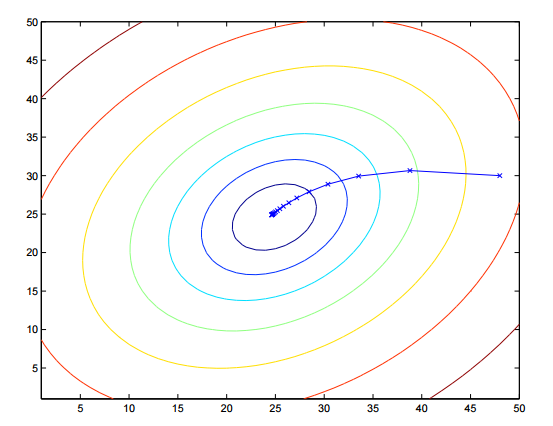
\includegraphics[scale=0.3]{ellipses.png}
 % ellipses.png: 553x426 px, 72dpi, 19.51x15.03 cm, bb=0 0 553 426
 \caption{Example of gradient descent}
 \label{fig:gradientDescent}
\end{figure}

%\paragraph{Algorithm 1: A gradient descent method}
To minimize Sparse Coding and dictionary learning's cost function we must use all our knowledge of mathematical optimization. There are many optimizations algorithm that can find an approximation which minimizes Sparse Coding and dictionary learning's cost function. Most famous one is the gradient descent, its simplicity of implementation and its results are no longer to be proved. It becomes an indispensable tool for Machine learning scientist.\\
The main idea is to find the local minimum of a cost function iteratively. At each step, the parameters are updating proportionally (this is step size, controlled by a learning rate $\lambda$) in the opposite direction of the gradient of the objective function (see figure \ref{fig:gradientDescent}).\\
As a reminder, our objective function is:
\begin{center}
 $\min\limits_{D} \frac{1}{n} \sum_{i=1}^{n}  \min\limits_{\gamma} \frac{1}{2} \| x_i - D \hspace{3px} \gamma \|_2^2 + \lambda \|\gamma_i \|_1$\\
\end{center}
In the dictionary learning step we assume that $\gamma$ is fixed and D variable. We can simplify our problem without all terms which do not depend on the dictionary D, let's define a function $f$ such that:
\begin{center}
 $f(D) = \min\limits_{D} \frac{1}{n} \sum_{i=1}^{n}\frac{1}{2} \| x_i- D \hspace{3px} \gamma_i \|_2^2 $\\
\end{center}
Then we can compute the gradient of $f(D)$:

\begin{center}
 $\bigtriangledown f(D) = \frac{1}{n} \sum_{i=1}^n (x_i -D \gamma_i)\gamma_i^{\intercal}$
\end{center}

\begin{algorithm}
\caption{Dictionary Learning: Gradient descent}
 \begin{algorithmic}
  \REQUIRE x, $\gamma$, $\alpha$
  \WHILE{D not converged}
        \STATE \textit{// Perform gradient descent update of D}
        \STATE $D = D - \alpha * (X-D\gamma)*\gamma^{\intercal}$
        \STATE \textit{// Renormalize columns of D}
        \FOR{ each column j of D}
            \STATE $D[:,j] = \frac{D[:,j]}{\|D[:,j]\|}$
        \ENDFOR
  \ENDWHILE
  \RETURN D
 \end{algorithmic}
\end{algorithm}

%\begin{lstlisting}[language=Python,frame=single]
%while D not_converged:
%    # Perform gradient update of D
%    D = D - alpha * (1/T)* sum((x - D h)* tranpose(h))
%    # Renormalize the columns of D
%    for each column D[:,j]:
%        D[:,j] = (D[:,j] / norm(D[:,j]))
%
%return D
%\end{lstlisting}

\subsubsection{Algorithm 2: Block-coordinate descent}

\begin{figure}[h]
 \centering
 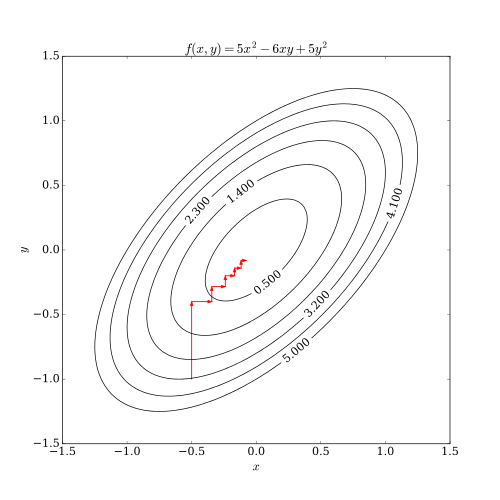
\includegraphics[scale=0.4]{Coordinate_descent.png}
 % Coordinate_descent.svg.png: 500x500 px, 72dpi, 17.64x17.64 cm, bb=0 0 500 500
 \caption{Example of Block-Coordinate descent}
 \label{fig:BlockCoordDescent}
\end{figure}

%We must minimize:
%\begin{center}
 %$\min\limits_{D} \frac{1}{T} \sum_{t=1}^{T}  \min\limits_{\gamma} \frac{1}%{2} \| x^{(t)} - D \hspace{3px} \gamma \|_2^2 $\\
%\end{center}
To avoid the learning rate there are other algorithms that can be applied instead of gradient descent. One of them is called Block-coordinate descent. The idea is to find the minimum of our objective's function for each direction in a cycle, in this case, a direction is a column of $D_{., j}$ (see figure \ref{fig:BlockCoordDescent}). Firstly, we have to set the gradient of $D_{., j}$ to zero.\\
\begin{center}
 $ \frac{1}{n}\sum_{i=1}^{n} (x_i - D \gamma_i)$ $\gamma_{[i,j]} = 0$\\ \vspace{0.4cm}
 We separe $D_{.,j}$ from the rest of D:\\
 $\iff 0 = \frac{1}{n}\sum_{i=1}^{n} (x_i - (\sum_{l \neq j}D_{.,l}$ $\gamma_{[i,l]}$ $ )$  $ - (D_{.,j}$ $\gamma_{[i,j]})$ ) $ \gamma_{[i,j]}$\\ \vspace{0.4cm}
 Our aim is to find the value of $D_{.,j}$, we must isolate $D_{.,j}$ :\\
 $\iff 0 = \frac{1}{n} \sum_{i=1}^{n}(x_i \gamma_{[i,j]} - (\sum_{l \neq j}D_{.,l}$ $\gamma_{[i,l]}$ $\gamma_{[i,j]} )$  $ - (D_{.,j}$ $\gamma^2_{[i,j]}))$\\ \vspace{0.2cm}
  $\iff 0 = (\sum_{i=1}^{n}(x_i \gamma_{[i,j]} - (\sum_{l \neq j}D_{.,l}$ $\gamma_{[i,l]}$ $\gamma_{[i,j]} )$  $) - ( \sum_{i=1}^{n}( D_{.,j}$ $\gamma_{[i,j]}^2)))$\\ \vspace{0.2cm}
  
  $ \iff \sum_{i=1}^{n}( D_{.,j}$ $\gamma^2_{[i,j]}) = \sum_{i=1}^{n}(x_i \gamma_{[i,j]} - (\sum_{l \neq j}D_{.,l}$ $\gamma_{[i,l]}$ $\gamma_{[i,j]} )$  $) $\\  \vspace{0.2cm}
  
  $\iff D_{.,j}  \sum_{i=1}^{n} \gamma^2_{[i,j]} = \sum_{i=1}^{n}(x_i \gamma_{[i,j]} - (\sum_{l \neq j}D_{.,l}$ $\gamma_{[i,l]}$ $\gamma_{[i,j]} )$  $) $\\ \vspace{0.2cm}
  
$\iff D_{.,j}  =\frac{1}{ \sum_{i=1}^{n} \gamma^2_{[i,j]}}\sum_{i=1}^{n}(x_i \gamma_{[i,j]} - (\sum_{l \neq j}D_{.,l}$ $\gamma_{[i,l]}$ $\gamma_{[i,j]})$  $) $\\ \vspace{0.2cm}

$\iff D_{.,j}  =\underbrace{\frac{1}{ \sum_{i=1}^{n} \gamma^2_{[i,j]}}}_{A_{j, j}} \underbrace{\sum_{i=1}^{n}(x_i \gamma_{[i,j]})}_{B_{., j}}  - \sum_{l \neq j}D_{., l}($ $\underbrace{\sum_{i=1}^{n} \gamma_{[i,l]} \alpha_{[i,j]} ) }_{A_{i,j}}$\\ \vspace{0.2cm}
$D_{., j} = \frac{1}{A_{j, j}}(B_{., j} - D A_{., j} + D_{., j}A_{j, j})$
\end{center}  

\begin{algorithm}
 \caption{Dictionary Learning: Block-coordinate descent}
 \begin{algorithmic}
    \REQUIRE X, $\gamma$
    \WHILE{ D not converged}
        \FOR{ each column j of D}
            \STATE \textit{// For each column D[:,j] perform update}
            \STATE $D[:,j] = \frac{1}{A[j,j]}  (B[:,j] - D  A[:,j] + D[:,j]  A[j,j])$
            \STATE \textit{// Normalization}
            \STATE $D[:,j] = \frac{D[:,j]}{\|D[:,j]\|}$
        \ENDFOR
    \ENDWHILE
    \RETURN D
 \end{algorithmic}

\end{algorithm}

%\begin{lstlisting}[language=Python,frame=single]
%while D not_converged:
%    # For each column D[:,j] perform updates
%    for each column D[:,j]:
%        D[:,j] = (1/A[j, j])*(B[:, j] - D A[:, j] + D[:, j] A[j, j])
%        # Normalization
%        D[:,j] = D[:,j]/norm(D[:,j])
%
%return D
%\end{lstlisting}

\subsubsection{Algorithm 3:  Online learning algorithm}
Today with the improvement of datasets size, it is impossible to train the dictionary over the entire dataset. To address this problem, machine learning scientist uses the online learning methods. Instead of learning on the entire dataset its update the model for each sample. In our case, we will update the dictionary after visiting each $x_i$. Mairal proposed  \cite{Mairal:2009:ODL:1553374.1553463} this online approach for the dictionary learning :
%\begin{itemize}
 %\item[$\bullet$]  Perform inference of $\gamma_i$ after visiting each $x_i$
% \item[$\bullet$]  Update running of the quantities required to update D: 
%        \begin{itemize}
%         \item B = $\beta B + (1 - \beta) x^{(t)}\gamma_i^T$
%         \item A = $\beta A + (1 - \beta)\gamma_i \gamma_i^T$
%        \end{itemize}
%\item[$\bullet$] Use current value of D as " warm start" to block-%coordinate descent (warm start $\iff$ With the previous value of D)
%\end{itemize}
%With $\beta$ a constant value use like a learning rate.

\begin{algorithm}
 \caption{Dictionary Learning: Online learning algorithm}
 \begin{algorithmic}
  \REQUIRE X, $\alpha$ (learning rate), T (number of iterations)
  \STATE $A = 0$, $B = 0$ (reset the ``past information"`)
  \STATE Initialize $D$ randomly (not to 0)
  \FOR{$t = 1$ to T}
    \STATE Infer code $\gamma$ from X
    \STATE $A = A + \gamma \gamma^{\intercal}$
    \STATE $B = B + X \gamma^{\intercal}$
    \FOR{$i = 1$ to n}
        \FOR{ each column j of D}
            \STATE $ D[:,j] = \frac{1}{A[j,j]}*(B[:,j] - D A[:,j] + D[:,j] A[j,j])$
            \STATE \textit{// Normalization}
            \STATE $D[:,j] = \frac{D[:,j]}{\|D[:,j]\|} $
        \ENDFOR
    \ENDFOR
  \ENDFOR
  \RETURN D
 \end{algorithmic}
\end{algorithm}


%\begin{lstlisting}[language=Python,frame=single]
%Initialize D # Not to 0 ! (To respect the constraint we define before)
%while D not_converged:
%    for each x:
%        Infer code h
%        #Update dictionary
%        A = A +  h * transpose(h)
%        B = B + x * transpose(h)
%        #Batch upgrade
%        #A = beta * A + ( 1 - beta ) * h * transpose(h)
%        #B = beta * B + ( 1 - beta ) * x * transpose(h)
%        while D not_converged:
%            for each column D[:,j]:
%                 D[:,j] = (1/A[j,j])*(B[:,j] - D A[:,j] + D[:,j] A[j,j])
%                # Normalization
%                D[:,j] = D[:,j]/norm(D[:,j]) 
%\end{lstlisting}
\paragraph{Optimizing the Algorithm}
In practice, it's possible to improve the convergence speed of this algorithm by using a Mini-batch extension: By drawing $\eta > 1 $ signals at each iteration instead of a single one. Thus we have:
\begin{center}
  \[    \left\{
                \begin{array}{ll}
                  A_t  = \beta A_{t-1} + \sum_{i=1}^{\eta} \alpha_{t,i}\alpha_{t,i}^{T}\\
                  B_t = \beta B_{t-1} + \sum_{i=1}^{\eta}x\alpha_{t,i}^{T}\\
                \end{array}
              \right.
  \]
\end{center}

With $\beta = \frac{\theta + 1 - \eta}{\theta +1}$, where $\theta = t \eta$ if $ t < \eta$ and $\eta^2 + t - \eta$ if $t \geq \eta$.


\subsubsection{Algorithm 4: K-SVD}
K-SVD is an algorithm proposed by Aharon, Elad, and Bruckstein \cite{1710377} that generalizes the K-mean clustering algorithm via a singular value decomposition (SVD) approach:

\begin{algorithm}
 \caption{K-SVD algorithm}
 \begin{algorithmic}
  \REQUIRE X
  \STATE Initialize D randomly
  \STATE  Ifer code $\gamma$ from X
   \FOR{ each column j of D}
    \STATE $GammaActive = \emptyset $
    \STATE $ActiveSet = \emptyset$
    \STATE $ErrorActiveSet = \emptyset$
    \FOR{i=1 to n}
        \IF{$\gamma_{[i,j]} \neq 0$}
            \STATE $GammaActive = GammaActive \bigcup gamma_{[i,j]}$
            \STATE $ActiveSet = ActiveSet \bigcup X_i$
            \STATE $temp = X_i$
            \FOR{ each $l$ such that $\gamma_{i,l} \neq 0$ and $l \neq j$}
                \STATE $temp = temp - D[:,l] $
            \ENDFOR
            \STATE $ErrorActiveSet = ErrorActiveSet \bigcup temp$
        \ENDIF
    \ENDFOR
    \STATE $D[:,j] = $ $\underset{D[:,j]}{\min}$ $\|ErrorActiveSet - D[:,j]*GammaActive)\|^2_2$   $
    \hspace{0.5cm}\Rightarrow$ This can be done by using SVD. 
  \ENDFOR
  \RETURN D
 \end{algorithmic}

\end{algorithm}

\newpage
\subsection{Application for MNIST dataset}
The MNIST database of handwritten digits, available from Yann Lecun's website. MNIST has a training set of 60,000 examples and a test set of 10,000 examples. It is a subset of a larger set available from NIST. The digits have been size-normalized and centred in a fixed-size image. In my test, I'll use 55000 examples from the training set (using Tensorflow datasets). These are $28 \times 28$ images. One way to evaluate the quality of our results is to compare the original data vs the reconstructed ones. 
\begin{figure}[h]
 \centering
 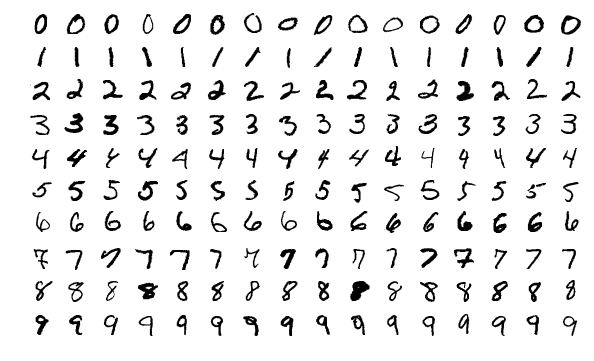
\includegraphics[scale=0.5]{MnistExamples.png}
 % MnistExamples.png: 594x361 px, 72dpi, 20.96x12.74 cm, bb=0 0 594 361
 \caption{Example of MNIST's handwitten digits}
\end{figure}
\subsubsection{Prototype}
My first task is to realise a Sparse Coding prototype to compute Sparse Coding on this dataset, using Python. The aim here is to understand the underlying principles of this method, you can found this prototype in \texttt{Code directory} of this repository as \texttt{SparseCoding.py}. \\
These are some results of this prototype: For time-saving, I used only 100 digits as input.

\subsubsection{SPAMS}
SPAMS (SPArse Modeling Software) is an optimization toolbox for solving various sparse estimation problems.
\begin{itemize}
 \item Dictionary learning and matrix factorization (NMF, sparse PCA, ...)
 \item Solving sparse decomposition problems with LARS, coordinate descent, OMP, SOMP, proximal methods
 \item Solving structured sparse decomposition problems (l1/l2, l1/linf, sparse group lasso, tree-structured regularization, structured sparsity with overlapping groups,...).
\end{itemize}
It is developed and maintained by Julien Mairal (Inria), and contains sparse estimation methods resulting from collaborations with various people: notably, Francis Bach, Jean Ponce, Guillermo Sapiro, Rodolphe Jenatton and Guillaume Obozinski.\\
You can find my code of Sparse Coding/Dictionary Learning on MNIST using SPAMS toolbox on my GitHub \texttt{test\_spams.py}.\\
\newpage
\paragraph{Test 1}
In the first test, I used 256 atoms, 2 000 iterations and $\lambda$ = 0.015 to learn the dictionary and the sparse coefficients. 
w\begin{figure}[h]
 \centering
 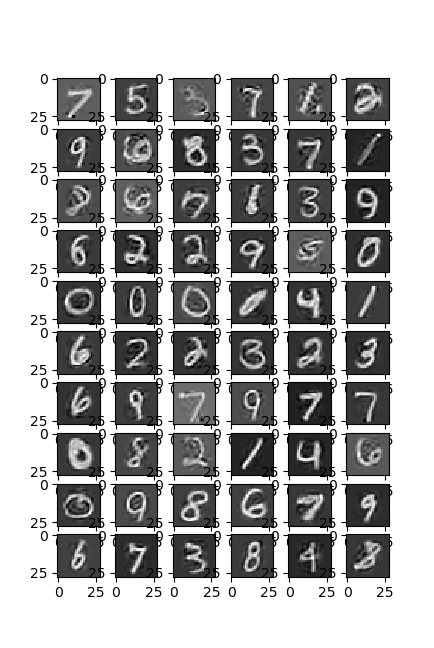
\includegraphics[scale=0.82]{../Results/SPAMS_X_ALL_K256/D.png}
 % D.png: 434x648 px, 100dpi, 11.02x16.46 cm, bb=0 0 312 467
 \caption{Few atoms of D}
\end{figure}

 \begin{figure}[h]
 \begin{subfigure}{.5\textwidth}
 \centering
 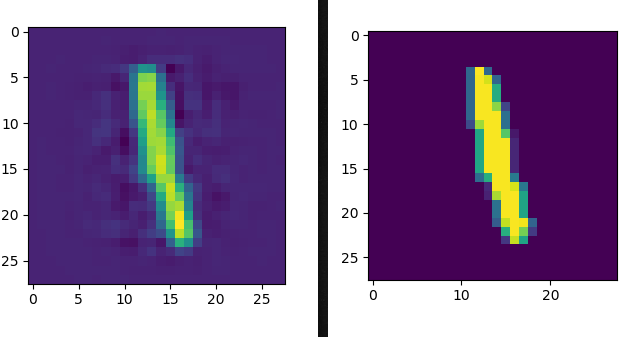
\includegraphics[scale=0.35]{../Results/SPAMS_X_ALL_K256/recons_1.png}
  \caption{Reconstructed 1 vs Original 1}
 % module-capteur-laser.jpg: 600x600 px, 72dpi, 21.17x21.17 cm, bb=0 0 600 600
 \end{subfigure}%
  \begin{subfigure}{.3\textwidth}
 \centering
 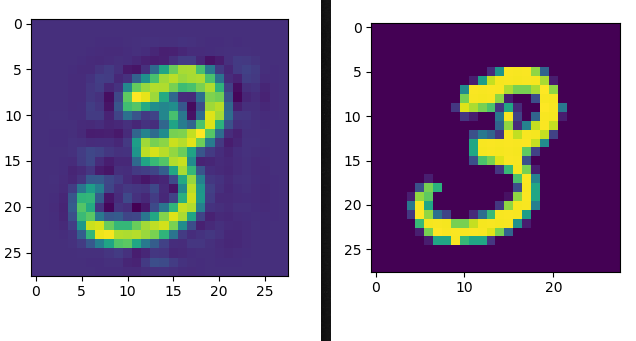
\includegraphics[scale=0.35]{../Results/SPAMS_X_ALL_K256/recons_3.png}
 % module-capteur-laser.jpg: 600x600 px, 72dpi, 21.17x21.17 cm, bb=0 0 600 600
  \caption{Reconstructed 3 vs Original 3}

 \end{subfigure}%
\end{figure}

\newpage

\paragraph{Test 2}In the second test I used 1024 atoms, 1 000 iterations and $\lambda = \frac{1.2}{\sqrt{m}}$ \cite{Mairal:2009:ODL:1553374.1553463} \textit{(In my case $\approx 0.0042857$)}.
\begin{figure}[h]
 \centering
 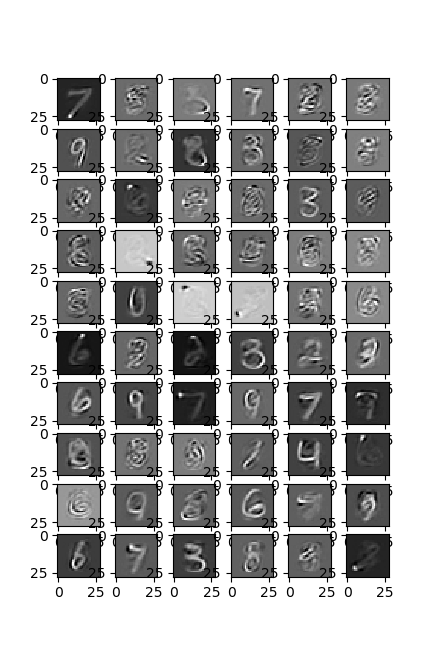
\includegraphics[scale=0.82]{../Results/SPAMS_X_ALL_K1024/D.png}
 % D.png: 1873x1022 px, 100dpi, 47.57x25.96 cm, bb=0 0 1349 736
 \caption{Few atoms of D}
\end{figure}
 \begin{figure}[h]
 \begin{subfigure}{.5\textwidth}
 \centering
 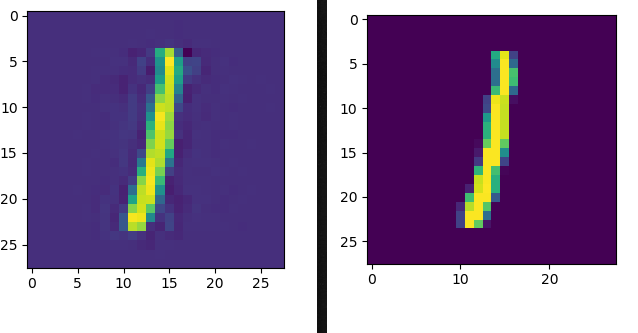
\includegraphics[scale=0.4]{../Results/SPAMS_X_ALL_K1024/lambdaopti_recons1.png}
  \caption{Reconstructed 1 vs Original 1}
 % module-capteur-laser.jpg: 600x600 px, 72dpi, 21.17x21.17 cm, bb=0 0 600 600
 \end{subfigure}%
  \begin{subfigure}{.3\textwidth}
 \centering
 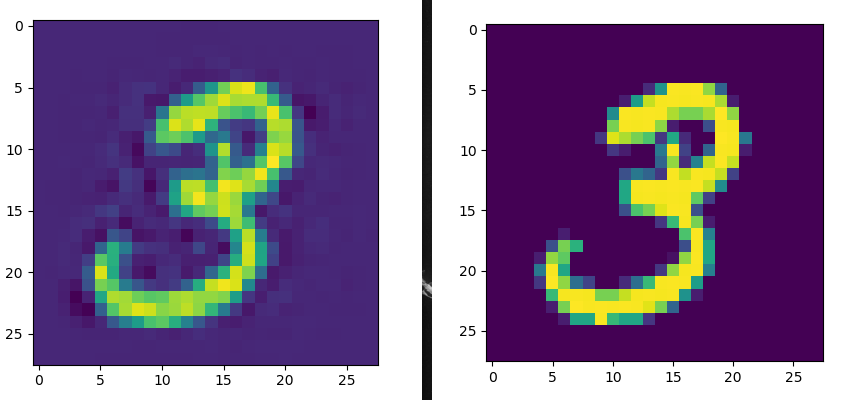
\includegraphics[scale=0.29]{../Results/SPAMS_X_ALL_K1024/lambdaopti_recons3.png}
 % module-capteur-laser.jpg: 600x600 px, 72dpi, 21.17x21.17 cm, bb=0 0 600 600
  \caption{Reconstructed 3 vs Original 3}

 \end{subfigure}%
\end{figure}
\newpage
\paragraph{Test 3} In the third test I used 1024 atoms, 1 000 iterations and $\lambda = 5$.
\begin{figure}[h]
 \centering
 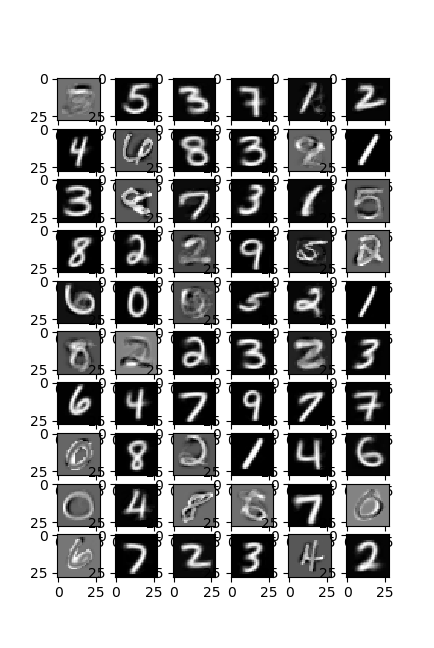
\includegraphics[scale=0.82]{../Results/SPAMS_X_ALL_K1024/D_lambdagrand.png}
 % D_lambdagrand.png: 936x994 px, 100dpi, 23.77x25.25 cm, bb=0 0 674 716
 \caption{Few atoms of D}
\end{figure}

 \begin{figure}[h]
 \begin{subfigure}{.5\textwidth}
 \centering
 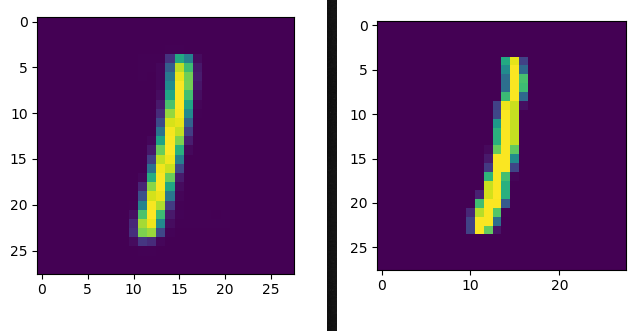
\includegraphics[scale=0.4]{../Results/SPAMS_X_ALL_K1024/lambdagrand_recons1.png}
  \caption{Reconstructed 1 vs Original 1}
 % module-capteur-laser.jpg: 600x600 px, 72dpi, 21.17x21.17 cm, bb=0 0 600 600
 \end{subfigure}%
  \begin{subfigure}{.3\textwidth}
 \centering
 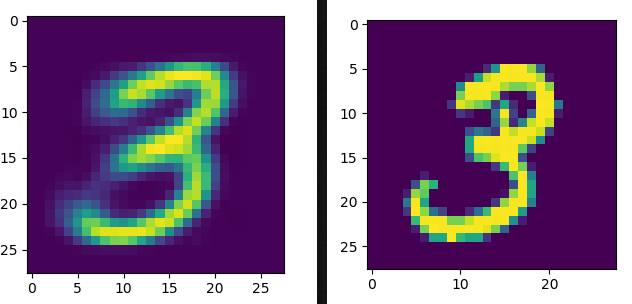
\includegraphics[scale=0.39]{../Results/SPAMS_X_ALL_K1024/lambdagrand_recons3.png}
 % module-capteur-laser.jpg: 600x600 px, 72dpi, 21.17x21.17 cm, bb=0 0 600 600
  \caption{Reconstructed 3 vs Original 3}

 \end{subfigure}%
\end{figure}

\newpage
\paragraph{Test 4} In the fourth test I used 2048 atoms, 1 000 iterations and $\lambda = \frac{1.2}{\sqrt{m}}$
\begin{figure}[h]
 \centering
 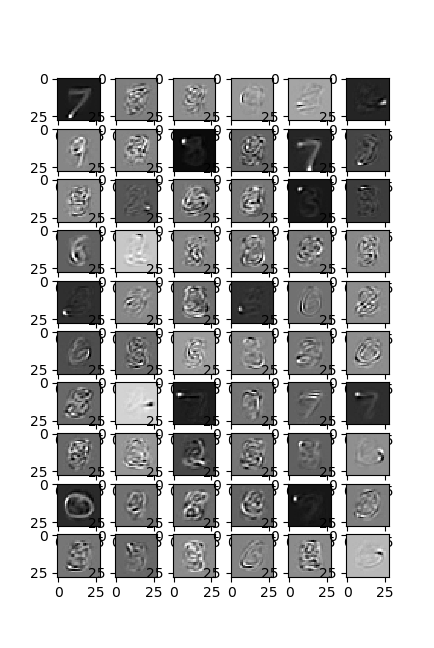
\includegraphics[scale=0.82]{../Results/SPAMS_X_ALL_K_2048/D_K2048.png}
 % D_K2048.png: 936x994 px, 100dpi, 23.77x25.25 cm, bb=0 0 674 716
 \caption{Few atoms of D}
 \end{figure}
 
  \begin{figure}[h]
 \begin{subfigure}{.5\textwidth}
 \centering
 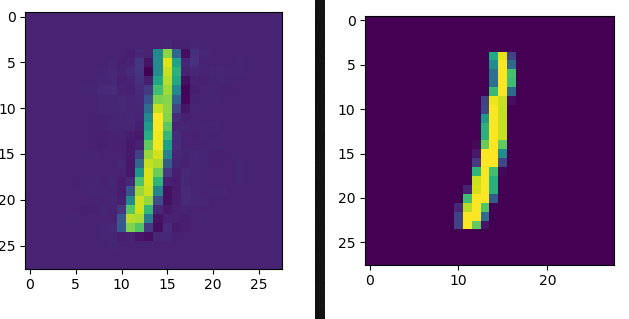
\includegraphics[scale=0.4]{../Results/SPAMS_X_ALL_K_2048/recons1.png}
  \caption{Reconstructed 1 vs Original 1}
 % module-capteur-laser.jpg: 600x600 px, 72dpi, 21.17x21.17 cm, bb=0 0 600 600
 \end{subfigure}%
  \begin{subfigure}{.3\textwidth}
 \centering
 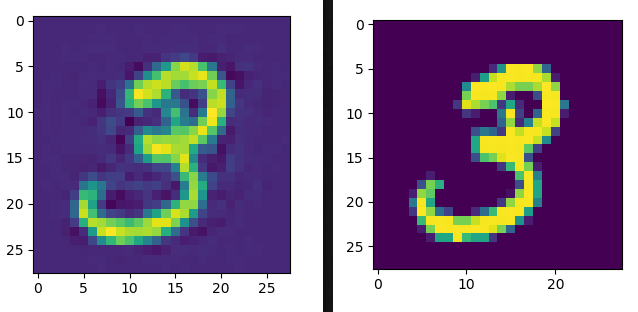
\includegraphics[scale=0.39]{../Results/SPAMS_X_ALL_K_2048/recons3.png}
 % module-capteur-laser.jpg: 600x600 px, 72dpi, 21.17x21.17 cm, bb=0 0 600 600
  \caption{Reconstructed 3 vs Original 3}

 \end{subfigure}%
\end{figure}

\newpage

%\subsection{Application for Lenna}

\begin{figure}[h]
 \centering
 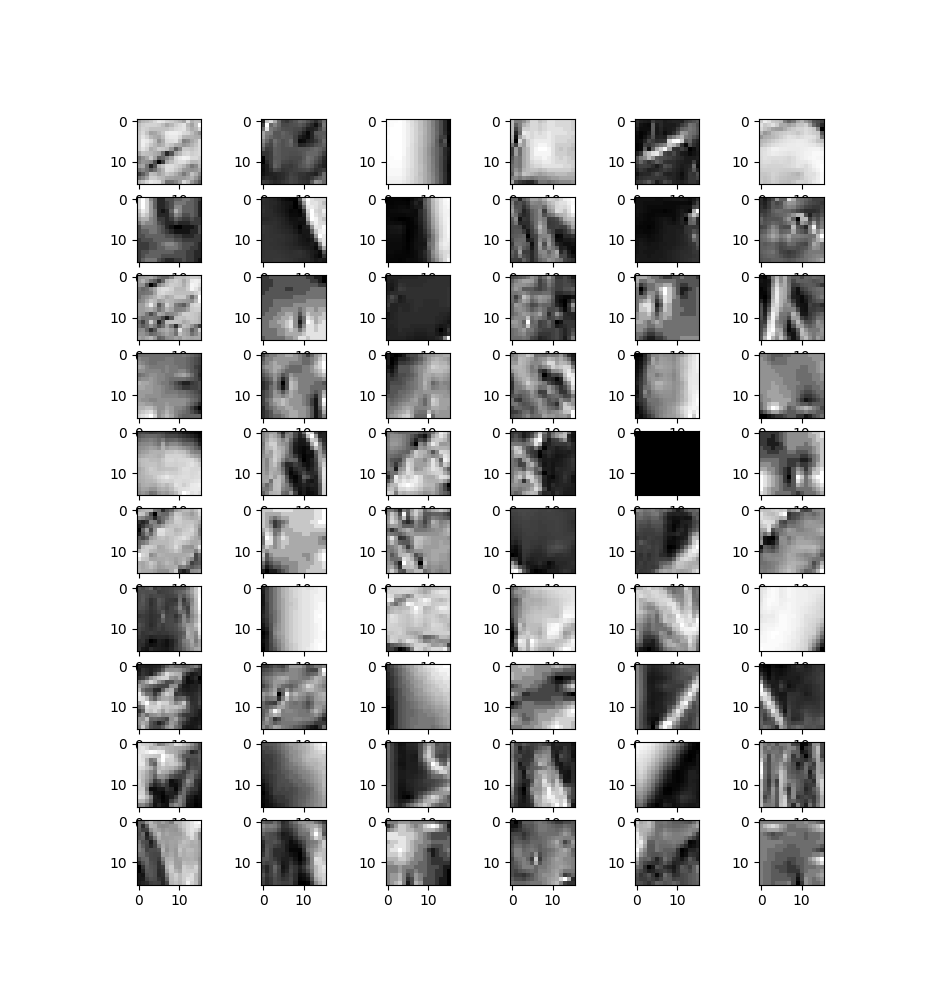
\includegraphics[scale=0.3]{../Results/Lenna/lenna_1024.png}
 % lenna_1024.png: 936x994 px, 100dpi, 23.77x25.25 cm, bb=0 0 674 716
 \caption{Some atoms of D when K = 1024}
\end{figure}
\begin{figure}[h]
 \centering
 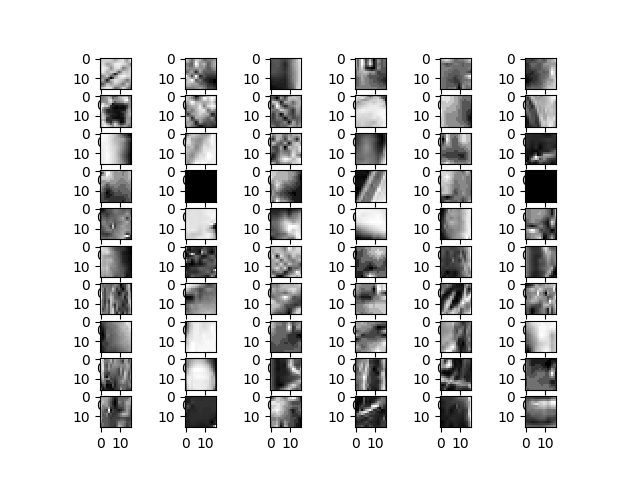
\includegraphics[scale=0.75]{../Results/Lenna/lenna_2048.png}
 % lenna_2048.png: 640x480 px, 100dpi, 16.26x12.19 cm, bb=0 0 461 346
 \caption{Some atoms of D when K = 2048}
\end{figure}
\newpage

%\subsection{Dictionary learning and sparse coding for unsupervised clustering}
\label{sec:Clustering}
Whereas the previous tests seem to have a good result, one question appears \\ \textit{What makes us confident about the fact that two close images (two handwritten 3 for example) have close coefficients representation h ?}\\
Sprechmann and Sapiro \cite{5494985} propose an algorithm to cluster datasets that are well represented in the sparse modelling framework with a set of K learned dictionaries. The main idea is, given a set of K dictionaries, find for each signal in the dictionary for which the "best" sparse decomposition is obtained, with :

\begin{center}
$\underset{D_i,C_i}{\min} \sum_{i=1}^{K} \sum_{x_j \in C_i} \mathcal{R}(x_j, D_i)$
 
\end{center}
Here $D_i \in \R^{n \times k_i}$ is the $k_i$ dictionary associated with the class $C_i$. $x_j \in \R^n$ are the input data and $\mathcal{R}$  a function that mesure how good the sparse decomposition is for the signal $x_j$ under the dictionary $D_i$. Sprechmann and Sapiro propose to use the cost function in the Lasso-type problem as $\mathcal{R}$ the measure of performance, $\mathcal{R}(x,D) = \|x - D\alpha\|^2_2 + \lambda \|\alpha\|_1$. The class $\mathcal{C}$ for a given signal x is found by solving $\mathcal{C}= \underset{j=1,..,K}{\argmin}$ $ \mathcal{R}(x,Dj) $.

\subsubsection{Dictionary learning for clustering}
Given a set of signals and number of classes, we want to find a set of K learned dictionaries that best represent x (the input data). \cite{5494985} formulate thus as an energy minimization problem and use the measure previously proposed,\\
\begin{center}
 $\underset{D_i,C_i}{\min} \sum_{i=1}^{K} \sum_{x_j \in C_i} \underset{\alpha_{ij}}{\min}\|x_j - D_i \alpha_{ij}\|^2_2 + \lambda\|\alpha_{ij}\|_1$
\end{center}
The optimization is carried out by solving one problem at time:
\begin{itemize}
 \item \textit{Assignement step:} The dictionaries are fixed and each signals is assigned to the cluster for which the best representation is obtained.
 \item \textit{Update step:} The new dictionaries are computed fixing the assignation found in the previous step.
\end{itemize}
One drawback of this algorithm is there is no guarantee of reach a global minimum. In this setting, repeated initialization are computationally expensive, thus we need a good initialization.

\subsubsection{Initialization}
The initialization can be given by a set of K dictionaries or as an initial partition of the data.\\
The main idea is to construct a similarity matrix and use it as the input for a spectral clustering algorithm. Let define $A = [\alpha_1,....,  \alpha_m]$ with $\alpha_j$ the sparse representation of each signal $x_j$. To obtain a good classification, we expect two signal to the same cluster to have decomposition that uses similar atoms. Thus we can compute two similarity matrix:
\begin{itemize}
 \item \textit{Clustering the signals :} Construct a similarity matrix $S_1 \in \R^{m \times m}$ which measure the similarity of two signals by comparing the corresponding sparse representation:\\
 $S_1 = |A|^T |A|$
 \item \textit{Clustering the atoms :} Construct a similarity matrix $S_2 \in \R^{k_0 \times k_0}$ ( with $D_0 \in \R^{n \times k_0}$) which represent the similarity of two atoms by comparing how many signals use them simultaneously and how they contribute in their sparse decomposition.\\
 $S_2 = |A||A|^T$
\end{itemize}
In this two case, the similarity matrixes are positive semidefinite and can be associated with a graph: $G_1 = \{X,S_1\}$ and $G_2 = \{D,S_2\}$ where the data (respectivly atoms) are the sets of vertexes with the corresponding $S_i$ as edge weights matrixes. This graph is partitioned using standard spectral clustering algorithm to obtain the initialization.\\
However, when K is large (the number of class), the performance of initial clusterization decreases. To fix this problem \cite{5494985} proposed to stat with the whole set as the only partition and at each itation we subdivise in two sets each of the current partitions, the procedure stops when the desired number of clusters is reached.



\newpage
\chapter{Discriminative Sparse Coding }
\label{chap:Discriminative}

\begin{figure}[h]
 \centering
 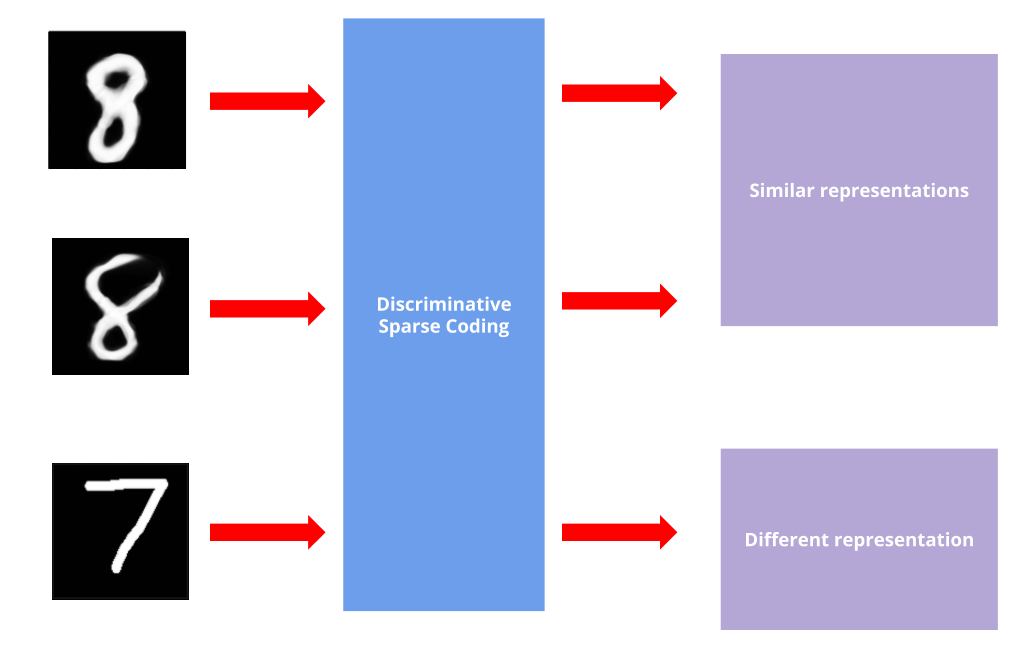
\includegraphics[scale=0.3]{discriminative.png}
 % discriminative.png: 1029x662 px, 72dpi, 36.30x23.35 cm, bb=0 0 1029 662
 \caption{Objective of discriminative Sparse Coding}
 \label{fig:discriminative}
\end{figure}
Generally, to get a discriminative sparse code, the first need is a discriminative dictionary. Indeed,  during the sparse coding step, if the dictionary is discriminative, the minimization of the lost function will tend to create the sparse code using the right atoms and be disadvantaged for the others atoms in term of reconstruction. The result will be a discriminative sparse code.\\
However, most methods of discriminative sparse coding are not unsupervised, because they use the label information during the training of the dictionary. \cite{8294264} enumerate some of these methods:
%One way to have discriminative Sparse coefficients is firstly to have a discriminative dictionary and there are serveral approach for discriminative Dictionary Learning enumerate by \cite{8294264}:
\begin{itemize}
 \item In presence of label:
    \begin{enumerate}
     \item Learn one dictionary per class
     \item Prune large dictionaries
     \item Jointly learn dictionary and classifier
     \item Embed class label into the learning of sparse coefficients
     \item Learn a histogram of dictionary elements over signal constituents
    \end{enumerate}

 \item For weakly supervised:\\
    Several max margin-based, non-convolutive, synthesis dictionary learning approaches
\end{itemize}
For the extraction of our features, we are only interested in two methods. We made this choice because both methods are state-of-the-art of discriminative Sparse Coding for feature's extraction (for classification purposes) and because they are simple to implement. We have chosen:
\begin{itemize}
 \item One Dictionary per class
 \item Embed class label into the learning of sparse coefficients, through a method named \textit{Label constitent K-SVD}.
\end{itemize}


%However in our problem of extract new features for speech we must compare each $\alpha$ with other, thus we must use only one dictionary.

\subsection{One dictionary per class}
The idea is to extend proposed method in  section \ref{sec:Clustering} by adding a term $\mathcal{Q}(D_i,D_j)$ that promotes incoherence between the differents dictionaries, e.g. this term encourage dictionaries to  be independent as possible :
\begin{center}
 $\underset{D_i, C_i}{\min} \sum_{i=1}^{K} \sum_{x_j \in C_i} \mathcal{R}(x_j,D_i) + \eta \sum_{i \neq j} \mathcal{Q}(D_i,D_j)$
\end{center}
For example we can take $\mathcal{Q}(D_i,D_j) = \|D^T_iD_j\|^2_F $ with F denotes Frobenius norm.

%\subsection{Supervised Dictionary learning SDL}
\subsubsection{Problem formulation}
In \cite{mairal:inria-00322431} the signal may belong to any of $p$ diffrent classes and they model the signal using a single shared D. They create a set of $p$ decision functions $g_i(x,\alpha,\theta)$ (i = 1,...,p). Where: \\
\begin{center}
  $g_i(x,\alpha,\theta) =     \left\{
                \begin{array}{ll}
                 gi > 0 $ if $x \in $ class i $\\
                g_i \leq 0$ otherwise$\\
                \end{array}
              \right.$
\end{center}
The vector $\theta$ parametrizes the model and will be jointly learned with the dictionary D. There are two kinds of models in this paper:\\
\begin{itemize}
 \item \underbar{Linear in $\alpha$:} $g_i(x,\alpha,\theta) = w_i^T \alpha + b_i $ where $ \theta = \{ w_i \in \R^k, b_i \in \R\}_{i=1}^p$
 \item \underbar{Bilinear in $x$ and $\alpha$: }$g_i(x,\alpha,\theta) = x^T W_i \alpha + b_i$ where $ \theta = \{W_i \in \R^{n \times k}, b_i \in \R\}_{i=1}^p$ 
\end{itemize}
They define a \textit{softmax} discriminative cost function as :
\begin{center}
 $\mathcal{C}_i(x_1,..., x_p) = log(\sum_{i=1}^p e^{x_j - x_i})$
\end{center}
Given x, a input signal, with $D$ and $\theta$ fixed, the supervised sparse coding problem for the class $p$ can be computing by :
\begin{center}
 $S^*_i(x,D,\theta) = \underset{\alpha}{\min}S_i(\alpha,x,D,\theta)$
\end{center}
where
\begin{center}
 $S_i(\alpha,x,D,\theta) = \mathcal{C}_i(\{g_j(x,\alpha,\theta)\}^p_{j=1}) + \lambda_0 \|x - D\alpha\|^2_2 + \lambda_1 \|\alpha\|_1$
\end{center}
Then, the classification problem can be compute by: 
\begin{center}
 
$i^*(x,D,\theta) = \underset{i=1,...,p}{\argmin}S^*_i(x,D,\theta)$
\end{center}

\subsubsection{Learning $D$ and $\theta$}
The most direct method for learning $D$ and $\theta$ is to minimize with respect to these (with $T_i$ a sample of input signals corresponding to the class i):
\begin{center}
 $\underset{D,\theta}{\min}(\sum_{i=1}^p \sum_{j \in T_i}S^*_i(x_j,D,\theta))+ \lambda_2 \|\theta\|^2_2$
\end{center}
With  $ \|\theta\|^2_2$ to prevent overfitting. They reffer to this model as SDL-G (Supervised Dictionary Learning - Generative) \cite{mairal:inria-00322431}.\\
A more discriminative approach is not only make $S^*_i$ small for signals with label i but also make the value of $S^*_j$ (with $i \neq j)$ greater than $S^*_i$. To do that they use the softmax cost function $\mathcal{C}_i$:
\begin{center}
  $\underset{D,\theta}{\min}(\sum_{i=1}^p \sum_{j \in T_i} \mathcal{C}_i(\{ S^*_l(x_j,D,\theta)\}^{p}_{l=1}))+ \lambda_2 \|\theta\|^2_2$
\end{center}
But this more difficult to solve, thus they adopt a mixed formulation with SDL-G :
\begin{center}
   $\underset{D,\theta}{\min}(\sum_{i=1}^p \sum_{j \in T_i} \mu \mathcal{C}_i(\{ S^*_l(x_j,D,\theta)\}^{p}_{l=1}) + (1-\mu)S^*_i(x_j,D,\theta))+ \lambda_2 \|\theta\|^2_2$
\end{center}
They refer to this model as SDL-D (Supervised Dictionary Learning - Discriminative). With $\mu$ which control the trade-off between reconstruction and discrimination.

\subsubsection{Optimization  procedure}
\paragraph{SDL-G}
When $\mu = 0$ or directly SDL-G have the same properties than classical dictionary learning techniques: Using block coordinate descent  consist of iterating between \textit{supervised sparse coding}, where $D$ and $\theta$ are fixed and optimize $\alpha$, and \textit{supervised dictionary update}, where  $\alpha$ is fixed but $D$ and $\theta$ are updated.
\paragraph{SDL-D} However the discriminative version of SDL (where $\mu \neq 0$) is not convex (even when $D$ and $\theta$ or $\alpha$ are fixed). To reach a local minimum for this problem, they have chosen a continuation method: Starting from the generative case and ending with the discriminative one.
\begin{figure}[h]
 \centering
 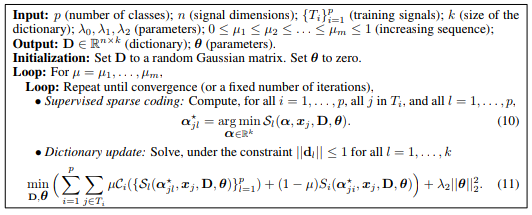
\includegraphics[scale=0.9]{SDL-D.png}
 % SDL-D.png: 532x215 px, 96dpi, 14.07x5.69 cm, bb=0 0 399 161
 \caption{SDL: Supervised dictionary learning Algorithm  \cite{mairal:inria-00322431}}
\end{figure}



\section{Label Consistent K-SVD}
\cite{6516503} proposed a supervised learning algorithm to learn a compact and discriminative dictionary for sparse coding. They add a new label consistency constraint ( ``discriminative sparse-code error") and combining reconstruction error and classification error to form a unified objective function that can be solved with the K-SVD algorithm.
%\subsection{Dictionary Learning for classification}
%A good classifier $f(x)$ can be obtained by determining its model parameters $W \in R^{m \times K} $ satisfying:
%\begin{center}
% $W = \underset{W}{\argmin} \underset{i}{\sum}\mathcal{L}\{h_i,f(x_i,W)\} + \lambda_1 \|W\|^2_F$
%\end{center}
%where: $m$ is the number of classes, $\mathcal{L}$ is the classification loss function (typically logistic loss function, suqare hinge loss, simple quadratic loss function), $h_i$ the label of $y_i$ and $\lambda_1$ a regularization parameters (which prevents overfitting).\\
%The objective function for learning $D$ and $W$ jointly can be :
%\begin{center}
 %$<D,W,\alpha> = \underset{D,W,\alpha}{\argmin} \|X -D\alpha\|^2_2 + \underset{i}{\sum}\mathcal{L}\{h_i,f(\alpha_i,W)\} + \lambda_1 \|W\|^2_F$  s.t.  $\forall i, \|\alpha_i\|_0 \leq T$ 
%\end{center}

%The sparse code $\alpha_i$ can be used as a feature descriptor of input signal $x_i$, then the risk minimization formulation can be written as:
%\begin{center}
 %$<D,W> = \underset{D,W}{\argmin}\underset{i}{\sum}\mathcal{L}\{h_i,f(\alpha^*(x_i,D),W)\} + \frac{\nu_1}{2}\|W\|^2_F$
%\end{center}
%Here D is not explicitly defined in the function but implicitlu in the sparse coding step ($\alpha^*(x_i,D)$ )

\subsection{Idea}
In a supervised setting, during the training phase, all the information about an input signal is given, including its label. The idea is to use this information to learn a discriminative dictionary. To do this, \cite{6516503} add a new consistency regularization term, a classification error and label consistency regularization term into the objective function:
\begin{center}
 $<D,\gamma> = \underset{D,\gamma}{\argmin} \|X - D\gamma\|^2_2 + \lambda \|\gamma\|_0 +\underset{Label\ consistent\ term}{\underbrace{\mu \|Q -AX\|_2^2 }} + \underset{Consistency\ term}{\underbrace{\beta\|H-WH\|_2^2}}$
\end{center}
%They refer to this two problem as LC-KSVD1 and LC-KSVD2 respectivly.
Where Q is the discriminative sparse codes of input signals X for classification, A is a linear transformation matrix, W is the classifier parameters and H is the labels corresponding to the input signal X.\\
This optimization function is called LC-KSVD2. But there is a variant of this method, called LC-KSVD1 which is the same function without the consistency term.\\
In our setting, we will use LC-KSVD1 because we do not want to train a classifier at this stage.
\subsection{LC-KSVD1}
Therefore, the objective function for dictionary learning is  defined as:
\begin{center}
 $<D,A,\gamma> = \underset{D,A,\gamma}{\argmin} \| X - D\gamma \|^2_2 + \mu \|Q -A\gamma\|^2_2 + \lambda\|\gamma\|_0$
\end{center}

Where $\mu$ controls the contribution between reconstruction and label consistency regularization. $Q = [q_1,...,q_N] \in \R^{K \times N}$.\\
Q is a discriminative sparse code corresponding to an input signal and the dictionary atoms, the nonzero values occur when $signal_i$ and $atom_i$ share the same label (figure \ref{fig:Q}).\\
Q is chosen by the user, in our setting we have chosen to match the same number of atoms for each class. It is then possible to have "empty" atoms that are not discriminative (white color's atom in figure \ref{fig:Q}).
\begin{figure}[h]
 \centering
 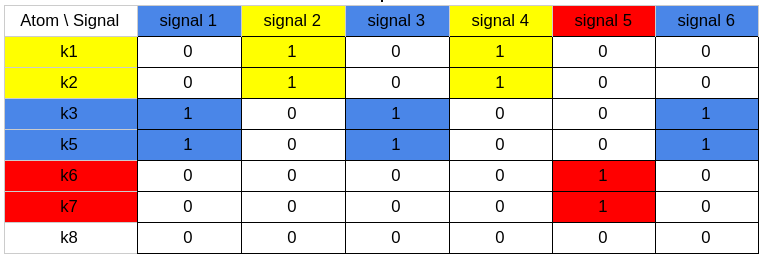
\includegraphics[scale=0.7]{LCKSVDTable.png}
 % Q_explications.png: 487x177 px, 96dpi, 12.88x4.68 cm, bb=0 0 365 133
 \caption{Example of Q, each color corresponding to a class (white color is the lack of classes). Signal 1,3 and 6 are from class 1; signal 2 and 5 from class 2 and signal 5 from class 3}
  \label{fig:Q}

\end{figure}
To use K-SVD algorithm it is necessary to  rewrite the previous equation:
\begin{center}
$ <D,A,\gamma> = \underset{D,A,\gamma}{\argmin} \| \begin{pmatrix} 
X  \\
\sqrt{\mu}Q
\end{pmatrix} -  \begin{pmatrix} 
D  \\
\sqrt{\mu}A
\end{pmatrix}\gamma \|^2_2\lambda \|\gamma\|_0$
\end{center}
We define $X_{new}  =  \begin{pmatrix} 
X  \\
\sqrt{\mu}Q
\end{pmatrix}$ and $D_{new} =  \begin{pmatrix} 
D  \\
\sqrt{\mu}A
\end{pmatrix}$. \\ \hspace{0.5cm}
It's important to note that the $D_{new}$ matrix is $L_2$ normalized. Now, it is possible to solve the minimization problem using the K-SVD algorithm:
\begin{center}
 $<D,A,\gamma> = \underset{D,A,\gamma}{\argmin} \| X_{new} - D_{new}\gamma \|^2_2 + \lambda \|\gamma\|_0$
\end{center}
However, it is impossible to use directly D and A  after employing the K-SVD algorithm. It is because D and A are $L_2$ normalized due to $D_{new}$. The desired $\hat{D}$ and $\hat{A}$ can be computed as follows:\vspace{0.5cm}\begin{center}
$\hat{D} = (
\frac{d_1}{\|d1\|_2}  ...  \frac{d_K}{\|d_K\|_2} 
)$   and $\hat{A} =
(\frac{a_1}{\|d_1\|_2}  ...  \frac{a_K}{\|d_K\|_2} 
)$
\end{center}
Label-Consistent K-SVD algorithm is given as follow:
\begin{algorithm}
 \caption{Label Consistent K-SVD 1 (LC-KSVD1)}
 \begin{algorithmic}
  \REQUIRE $X, Q, \lambda_1$
  \STATE $D_0$ = KSVD($X, \lambda_1$)
  \STATE $A_0 = Q  X^{\intercal} (X  X^{\intercal} + \lambda_2  I)^{-1}$
  \STATE $\gamma_0$ = OMP($D_0, X, lambda_1$)
  \STATE $X_{new}  =  \begin{pmatrix} 
    X  \\
    \sqrt{\mu}Q
    \end{pmatrix}$
  \STATE $D_{new} =  \begin{pmatrix} 
    D  \\
    \sqrt{\mu}A
    \end{pmatrix}$
  \STATE $ D = $ KSVD($D_{new}, X_{new}, \lambda_1)$
  \STATE $\hat{D} = (
\frac{d_1}{\|d1\|_2}  ...  \frac{d_K}{\|d_K\|_2} 
)$
\STATE $\hat{A} =
(\frac{a_1}{\|d_1\|_2}  ...  \frac{a_K}{\|d_K\|_2} 
)$
\RETURN $\hat{D}, \hat{A}$
 \end{algorithmic}

\end{algorithm}

%\vspace{0.5cm}
%\begin{lstlisting}[language=Python,frame=single]
%Input: X, Q, lambda1, K
%Output: D, A
%===========================================================================
%D_0 = K-SVD(X,lambda1)
%A_0 = Q * tranpose(X) * inv(X*tranpose(X) + lamba2 * Id)
%h_0 = omp(Dnew,Xnew,lambda1)

%Initialize Xnew and Dnew
%D = K-SVD(Dnew,Xnew,lambda1)

%Extract D, A
%return D, A
%\end{lstlisting}
%\vspace{0.5cm}
%With $A_0 = Q X^T (XX^T + \lambda_2 I)^{-1}$
%\vspace{0.5cm}\\
%In our case we don't want to train the classifier, we only want to find new features. This is why we only apply LC-KSVD1.\\
%You can find my Python code of  LC-KSVD1 on MNIST in my Github repository: \texttt{LC-KSVD.py}

\newpage

\subsection{Application on MNIST}
For k = 1024 and $\mu = 5$:

\begin{figure}[h]
 \centering
 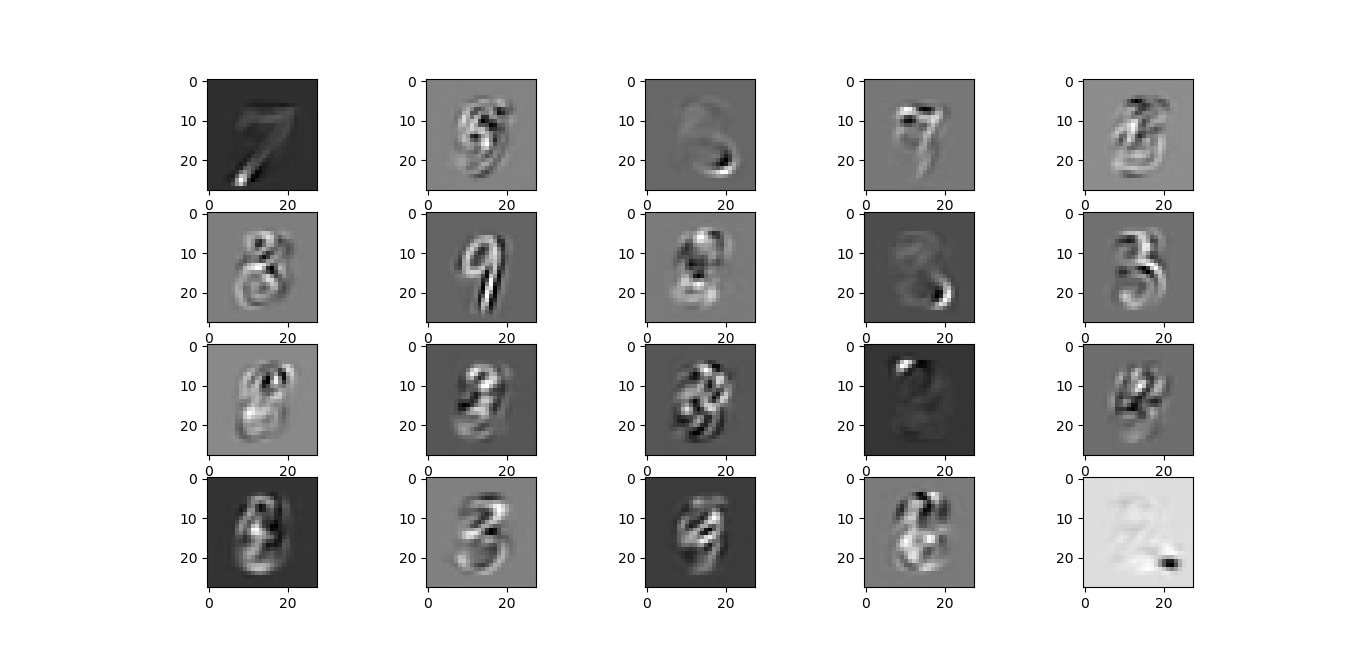
\includegraphics[scale=0.5]{../Results/LC-KSVD_X_ALL_K_1024/D.png}
 % D.png: 1366x660 px, 100dpi, 34.70x16.76 cm, bb=0 0 984 475
 \caption{Examples of D's atoms}
\end{figure}

\begin{figure}[h]
 \centering
 \includegraphics[scale=0.5]{../Results/LC-KSVD_X_ALL_K_1024/repartition_h.png}
 % répartition_h.png: 681x651 px, 100dpi, 17.30x16.54 cm, bb=0 0 490 469
 \caption{Sparse coefficients repartition}
\end{figure}
\begin{figure}[h]
 \centering
 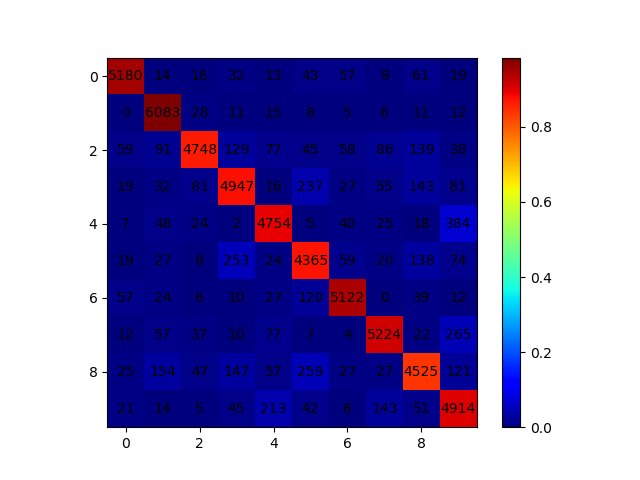
\includegraphics[scale=0.72]{../Results/LC-KSVD_X_ALL_K_1024/confusion_matrix_train.png}
 % confusion_matrix_train.png: 640x480 px, 100dpi, 16.26x12.19 cm, bb=0 0 461 346
 \caption{Kmeans classification on A$\alpha$ from the trainning dataset}
\end{figure}


 \begin{figure}[h]
 \begin{subfigure}{.5\textwidth}
 \centering
 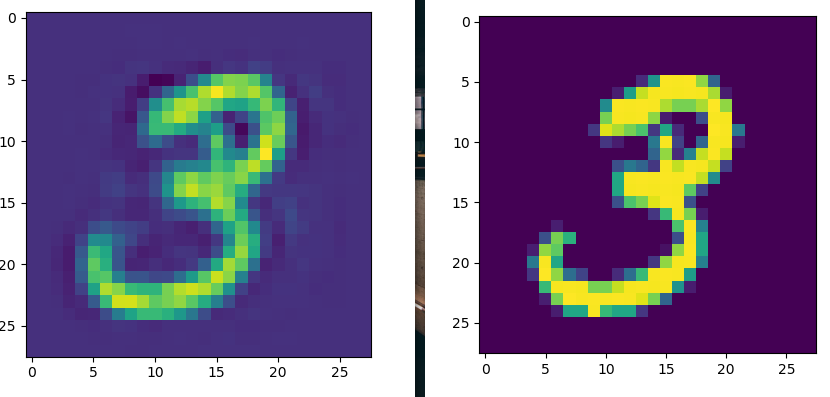
\includegraphics[scale=0.29]{../Results/LC-KSVD_X_ALL_K_1024/3_recons.png}
  \caption{Reconstructed 3 vs Original 3}
 % module-capteur-laser.jpg: 600x600 px, 72dpi, 21.17x21.17 cm, bb=0 0 600 600
 \end{subfigure}%
  \begin{subfigure}{.3\textwidth}
 \centering
 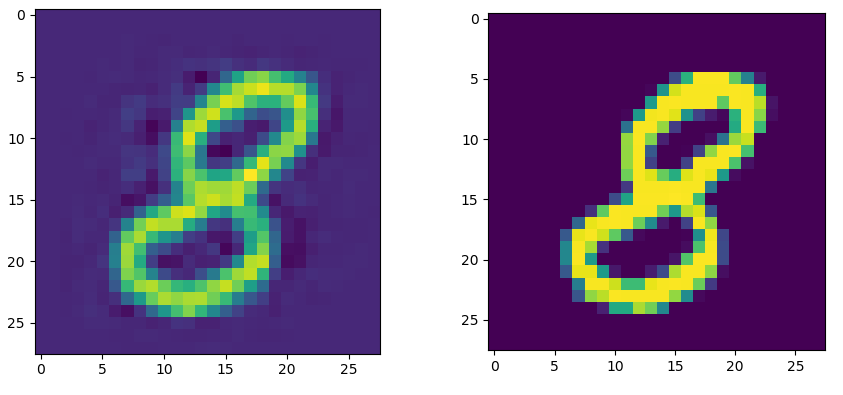
\includegraphics[scale=0.29]{../Results/LC-KSVD_X_ALL_K_1024/8_recons.png}
 % module-capteur-laser.jpg: 600x600 px, 72dpi, 21.17x21.17 cm, bb=0 0 600 600
  \caption{Reconstructed 8 vs Original }

 \end{subfigure}%
\end{figure}

\begin{figure}[h!]
 \centering
 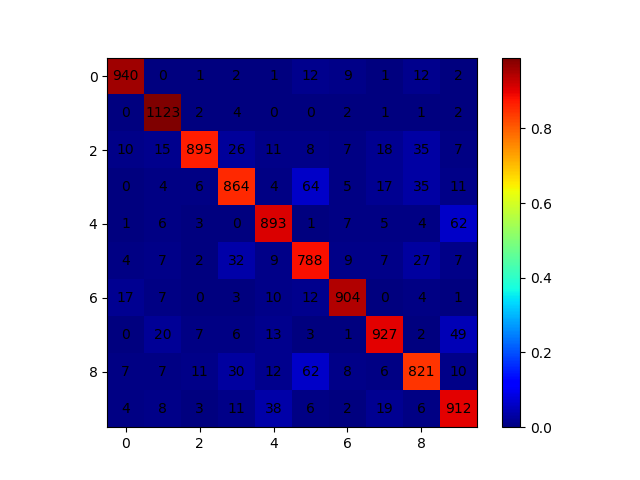
\includegraphics[scale=0.72]{../Results/LC-KSVD_X_ALL_K_1024/confusion_matrix_test.png}
 % confusion_matrix_test.png: 640x480 px, 100dpi, 16.26x12.19 cm, bb=0 0 461 346
 \caption{Kmeans classification on A $\alpha$ from the test dataset w}
\end{figure}

%\newpage
%\newpage
%
\subsection{Application on ``voyelle'' dataset }
We have for our experiments some audio signals that have been recorded in a studio. The speaker pronounces 10 vowels. There are 100 occurrences of each vowel (\textit{aa, ee, eh, eu, ii, oe, oh, oo, uu, yy}). Each signal is of 1024 sample.\\
A cepstral parametrization has been extracted from these samples, and a PCA has been done to reduce the data's dimension to  2 and 12. \vspace{0.5cm} \\
First, we focus our research on 2 dimension dataset. There are 10 classes which correspond to 10 vowels.\newline
\begin{figure}[h]
 \centering
 \includegraphics[scale=1]{../Results/Voyelles/voyelle_2.png}
 % voyelle_2.png: 445x648 px, 100dpi, 11.30x16.46 cm, bb=0 0 320 467
 \caption{Kmean classification on A$\alpha$ from the train dataset}
\end{figure}
 \\
\textit{Note: Here there is bad cluster identification (this is why we don't have a perfect diagonal matrix), however, the result is the same: In this case, our method is bad for classification because on the same row or column there is sometimes a bad repartition. It's due to the length of our input vector (2 dimensional vector), which is not enough to get the good result for classification using this method of Sparse representation of the signal.} \vspace{0.5cm}
\newpage
Then we focus our approach on 12 dimension dataset:
\begin{figure}[h]
 \centering
 \includegraphics[scale=0.49]{../Results/Voyelles/voyelle_13_train.png}
 % voyelle_13_train.png: 800x630 px, 100dpi, 20.32x16.00 cm, bb=0 0 576 454
 \caption{Kmean on data12 train set}
\end{figure}
\begin{figure}[h]
 \centering
 \includegraphics[scale=0.5]{../Results/Voyelles/voyelle_13_test.png}
 % voyelle_13_test.png: 1366x660 px, 100dpi, 34.70x16.76 cm, bb=0 0 984 475
 \caption{Kmean on data12 test set}
\end{figure}
 \begin{figure}[h]
 \centering
 \includegraphics[scale=0.45]{../Results/Voyelles/VoyellesAhRepartition.png}
 % VoyellesAhRepartition.png: 1366x660 px, 100dpi, 34.70x16.76 cm, bb=0 0 984 475
 \caption{ Four examples of A$\alpha$ from two different classes (orange and blue : Class 1, red and green: Class 2)}
\end{figure}
\newpage
\subsection{Discussion}
LC-KSVD perform well on our two datasets (MNIST and voyelle) when the input data are large enough (when input equal 2 we can see we get a bad result of clusterization). With this method we have two dictionaries: 
\begin{enumerate}
 \item \textbf{D} : A reconstructive dictionary
 \item \textbf{A}: A discriminative dictionary
\end{enumerate}
Using \textbf{A} we get a new representation of our input, a discriminative one, that we can put in the input of classifier to get a good classification.\\
However, this method works well on non-shift variant signals. When we have shift variant signal this method will fail to get a good discriminative representation i.e. If we have the same signal but delay with $\delta$, LC-KSVD will fail to get a close representation of the two signals.

\newpage
\chapter{Convolutional Sparse Coding}
\label{chap:Conv}
\subsection{Idea}
There are other algorithms like Efficient Shift-Invariant Dictionary learning which refers to the problem of discovering a set of latent basis vectors that capture informative \textit{local patterns} at different locations of the input sequences and not in all input sequences \cite{Zheng:2016:ESD:2939672.2939824}, to do that, we will use Convolutional Sparse Coding method.  
\subsection{Problem formulation}
Instead  of decomposing a signal as the $x = Dh$, Convolutional Sparse Coding (CSC) is the summation of convolutions between the feature map and the corresponding filter.
\begin{center}
 $X = \sum_{i=1}^{m} d_i * Z_i$\\  \vspace{0.4cm}
  $\underset{d, z}{\argmin}  \frac{1}{2} \| x - \sum_{k=1}^{K} d_k * z_k \|_2^2 + \beta \|z_k \|_1$\\

\end{center}
This new approach assume the ensemble of input vectors X are independent of one another. But the complexity of convergence is dramatically increase.
Bristow propose an Augmented Lagrangian and the used of  Alternative Direction Method of Multipliers (ADMM) \cite{6618901} to solve this problem. His approach is based on three key points:
\begin{itemize}
 \item The use of ADMM
 \item The convolution subproblem can be solved efficiently (and explicitly) in the Fourier domain (instead of temporal domain)
\item The use of quad-decomposition of the objective into four subproblems (that are convex)
\end{itemize}
In this approach, to solve a Convolutional Sparse Coding problem we introduce two auxilliary variables: \textbf{t} and \textbf{s} and posing the objective in the Fourier domain:
\begin{center}
$\underset{d, s, z, t}{\argmin} \hspace{0.4cm} \frac{1}{2D} \| \hat{x} - \sum_{k=1}^{K} \hat{d}_{k} \odot \hat{z}_k \|^2_2 + \beta \sum_{k=1}^{K} \|t_k\|_1$\\
subject to $\hspace{0.4cm} \|s_k\|^2_2 \leq 1 $ for k = 1.. K\\
                $ \hspace{2.4cm}s_k = \Phi^T \hat{d}_k$ for k = 1..K\\
                $\hspace{1.9cm}z_k = t_k$ for k = 1..K
\end{center}
With $\Phi$ a D $\times$ M submatrix of the Fourier matrix $F = [\Phi,\Phi_\bot]$. In this formulation $\hat{d}_k$ is a D dimensional vector whereas in the original formulation $d_k \in \R^M$  is of a significantly smaller dimensionality to $M \ll D$  corresponding to its smaller spatial support. 


\subsection{Solve the minimization problem}
\subsubsection{Augmented Lagrangian}
We handle the introduction of new equality constraints through an augmented Lagrangian approach \cite{6618901}:\\
\begin{center}
$ \hspace{-8cm} \mathcal{L}(d,s,z,t, \lambda_s, \lambda_t) =$ \\

$ \frac{1}{2D} \| \hat{x} - \sum_{k=1}^{K} \hat{d}_k \odot \hat{z}_k \|^2_2 + \beta \|t\|_1$\\
$ + \lambda^{T}_s(s-[\Phi^T \otimes I_K]\hat{d}) + \lambda^{T}_t (z - t)$\\
$ \hspace{-1.7cm}+ \frac{\mu_s}{2} \| s - [\Phi^T \otimes I_K]\hat{d}\|^2_2$\\
$ \hspace{-3.2cm}+ \frac{\mu_s}{2} \|z-t\|^2_2$
\end{center}
\subsubsection{Quad-decomposion of the objective}
We decompose our objective into four convex subproblems:


\paragraph{Subproblem z}:\vspace{0.5cm}\\
$z^* = \underset{z}{\argmin}$ $\mathcal{L}(z,d,s,t, \lambda_s, \lambda_t)$\\
$ = \mathcal{F}^{-1}\{\underset{z}{\argmin} \frac{1}{2}\|\hat{x} - \hat{D} \hat{z}\| + \hat{\lambda}_t^T(\hat{z}  - \hat{t}) + \frac{\mu_t}{2}\|\hat{z} - \hat{t}\|^2_2\}$\\
$= \mathcal{F}^{-1}\{(\hat{D}^T \hat{D} + \mu_tI)^{-1}(\hat{D}^T \hat{x} +  \mu \hat{t} - \hat{\lambda}_t)\} \vspace{0.6cm}$\\
Where $\hat{D} = [diag(\hat{d}_1),...,diag(\hat{d}_K)]$


\paragraph{Subproblem t}:\vspace{0.5cm}\\
$t^* =  \underset{t}{\argmin}$ $ \mathcal{L}(t,d,s,z,\lambda_s,\lambda_t)$\\
$ =  \underset{t}{\argmin}\frac{\mu_t}{2} \|z - t\|^2_2 + \lambda_t^T(z-t) + \beta\|t\|_1$\\
Unlike subproblem z, the solution to t cannot be efficiently computed in the Fourier domain (since $L_1$ norm is not rotaiton invariant). Solving t requires projecting $\hat{z}$ and $\hat{\lambda}_t$ back into the spatial domain. If this equation does not contain any rotations of the data, each element of t can be solved independently:\vspace{0.3cm}\\
$t^* =  \underset{t}{\argmin} \beta |t| + \lambda_t(z-t) + \frac{\mu}{2}(z-t)^2$\\
Where the optimal value of each t can be found using shrinkage function:\vspace{0.5cm}\\
$t^* = sign(z + \frac{\lambda_t}{\mu_t}) . max\{|z + \frac{\lambda_t}{\mu_t} | - t , 0\}$

\paragraph{Subproblem d}:\vspace{0.5cm}\\
$d^* =  \underset{s}{\argmin}$ $  \mathcal{L}(d,s,z,t,\lambda_s, \lambda_t)$\\ 
$ = \mathcal{F}^{-1} \{ \underset{\hat{d}}{\argmin}\frac{1}{2} \|\hat{x} - \hat{Z}\hat{d}\|^2_2 + \hat{\lambda}_s^T(\hat{d}- \hat{s}) + \frac{\mu}{2}\|\hat{d} - \hat{s}\|^2_2\}$\\
$ = \mathcal{F}^{-1}\{(\hat{Z}^T \hat{Z} + \mu_s I)^{-1} (\hat{Z}^T \hat{x} + \mu_s \hat{s} - \hat{\lambda}_s)\}$
\paragraph{Subproblem s}:\vspace{0.5cm}\\
$s^* =\underset{s}{\argmin}$ $  \mathcal{L}(d,s,z,t,\lambda_s, \lambda_t) $\\
$  = \underset{s}{\argmin}$ $\frac{\mu_s}{2} \|\hat{d} - [\Phi^T \otimes I_K]s\|^2_2 + \hat{\lambda}_s^T(\hat{d} - [\Phi^T \otimes I_K]s)$\\
Solving this equation as it is a quadratically constrained quadratic programming problem (QCQP).  Due to the Kronecker product with the identity matrix $I_K$ it can be broken down into K independent problems:\\
$s^*_k = \underset{s_k}{\argmin}$ $\frac{\mu_s}{2} \|\hat{d}_k  - \Phi^T s_k\|^2_2 + \hat{\lambda}_{sk}^T(\hat{d}_k - \Phi^T s_k)$\\
Futher, since $\Phi$ is orthonormal projectiong the optimal solution to the unconstrained problem cab be found efficiently through:\\

\begin{center}
  $s^* =     \left\{
                \begin{array}{ll}
                 \|\tilde{s}\|^{-1}_2 \tilde{s}_k $ , if $ \|\tilde{s}\|^{-1}_2 \geq 1\\
                \tilde{s}_k $ otherwise$\\
                \end{array}
              \right.$
\end{center}
where,
\begin{center}
 $\tilde{s}_k = (\mu_s \Phi \Phi^T)^{-1} (\Phi \hat{d}_k + \Phi \hat{\lambda}_{sk})$
\end{center}

Finally the solution to this equation can be found using :\\
$\tilde{s}_k = \mathcal{M}\{\frac{1}{\mu_s} \sqrt{D}^{-1}(  \mathcal{F}^{-1}\{\hat{d}_k\} +  \mathcal{F}^{-1}\{\hat{\lambda}_{sk}\}  ) \}$\\


\subsubsection{Lagrange Multiplier Update}
\begin{center}
 $\lambda^{(i+1)}_{t} \leftarrow \lambda^{(i)}_{t}  + \mu_t(z^{(i+1) - t^{(i+1)}}) $\\
 $\lambda^{(i+1)}_{s} \leftarrow \lambda^{(i+1)}_{s}  +\mu_s(d^{(i+1) - s^{(i+1)}}) $\\
\end{center}

\subsubsection{Penalty update}
Convergence may be reach if $\mu^{(i)} \rightarrow \infty$:

\begin{center}
  $\mu^{(i+1)} =     \left\{
                \begin{array}{ll}
                 \tau \mu^{(i)}$ if $\mu^{(i)} < \mu_{max} \\
                \mu^{(i)}$ otherwise$\\
                \end{array}
              \right.$
\end{center}

\section{SPORCO}
SPORCO \footnote{https://sporco.readthedocs.io/en/latest/index.html} (\textbf{SP}arse \textbf{O}ptimization \textbf{R}esearch \textbf{CO}de) is a Python package developed by  B. Wohlberg for solving optimization problem with sparsity problem  \cite{wohlberg-2017-sporco, wohlberg-2016-sporco}. These consist primarily of sparse coding and dictionary learning problems but there is also support for other problems such as:
\begin{itemize}
 \item Convolutional sparse coding
 \item ADMM
 \item Iterative shrinkage
 \item Total variation regularisation
 \item Robust PCA
 \item \dots
\end{itemize}
We will use Convolutional Sparse coding algorithm from this toolbox to confirm that CSC is shift-invariant.
\newpage
%\subsection{Application on random images}
In this section we show result for applying unsupervised Convolutional Sparse Coding (denoted as CSC) presented before on 7 random images, 6 for our train and 1 for our test.
\begin{figure}[h]
 \centering
 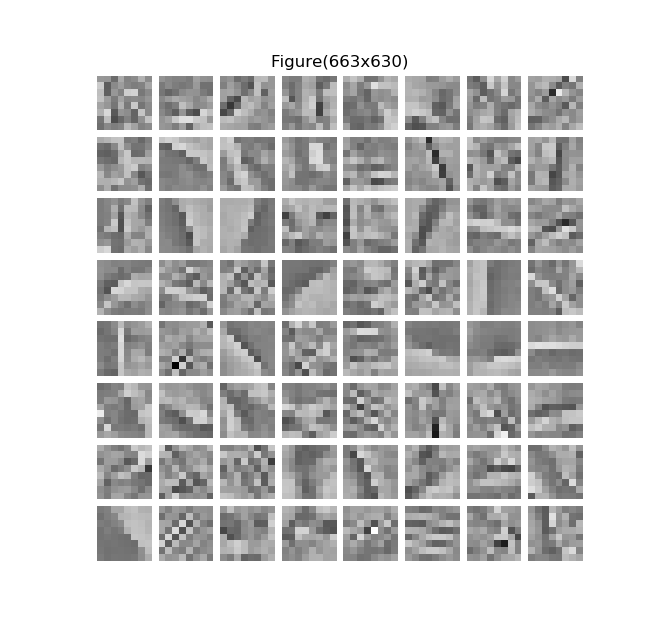
\includegraphics[scale=0.6]{../Results/SPORCO_test_img/Figure_2.png}
 % Figure_2.png: 663x630 px, 100dpi, 16.84x16.00 cm, bb=0 0 477 454
 \caption{Dictionary learned with 6 random images}
\end{figure}
\begin{figure}[h]
 \centering
 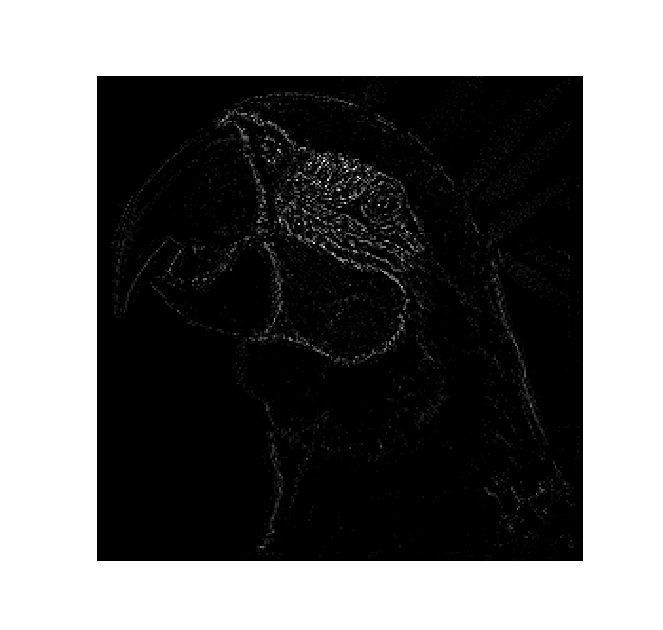
\includegraphics[scale=0.455]{../Results/SPORCO_test_img/activations.png}
 % activations.png: 663x630 px, 100dpi, 16.84x16.00 cm, bb=0 0 477 454
 \caption{Activation}
\end{figure}
\begin{figure}[h]
 \centering
 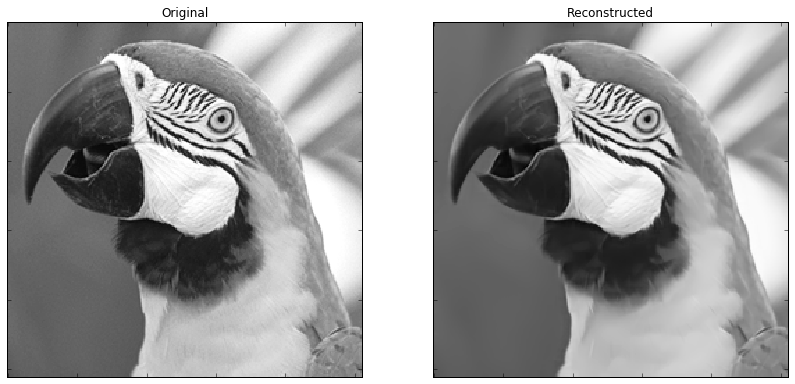
\includegraphics[scale=0.4]{../Results/SPORCO_test_img/recons.png}
 % recons.png: 795x384 px, 72dpi, 28.05x13.55 cm, bb=0 0 795 384
 \caption{Original image vs Reconstructed one}
\end{figure}


\newpage
\section{Experimentation details}
\subsection*{Application of Convolutional Sparse Coding on MNIST}
In this section, we show the result of applying unsupervised Convolutional Sparse Coding (denoted as CSC) previously presented in MNIST dataset.\\
Here, it's useless to have more than $2* Signal\_size$ not represent the number of atoms but its represent the number of filters, and we need fewer filters than atoms in the traditional Sparse Coding. Arbitrationally, we chose 64 filters of (8 $\times$ 8), this is not recommended to use filters larger than (7$\times$7) for MNIST dataset  \cite{best-practices-for-convolutional-neural-networks-applied-to-visual-document-analysis} however in our case we want to get more discriminant filters, so using larger filters is the solution.\\

\begin{figure}[h]
 \centering
 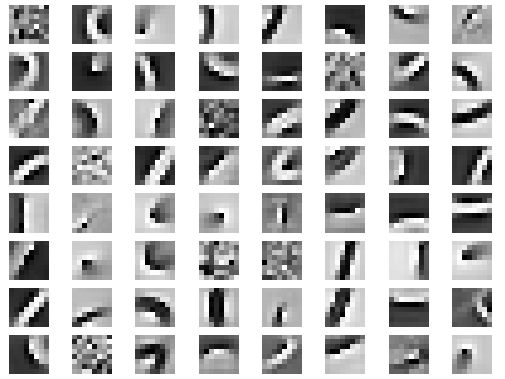
\includegraphics[scale=1]{CSC_D.png}
 % CSC_D.png: 640x480 px, 100dpi, 16.26x12.19 cm, bb=0 0 461 346
 \caption{Filters from the convolutional dictionary}
 \label{fig:CSC_D}
\end{figure}
As explained above,larger is the filter's size, more complex the pattern is. In our filters, we learned different types of curves (see figure \ref{fig:CSC_D}) that are more adapted to MNIST semantics. When we tried on smaller filter dimension we got  Gabor-like filters.\\
In order to use the activation maps obtained to make the classification, we want more complex models as possible. \\
In case of figure \ref{fig:CSC_D}, these curves are easy to find in some of our Latin/Western/Arabic numbers and are discriminative. For example, the second filter in figure \ref{fig:CSC_D} cannot be present for a handwritten 1.\\


\begin{figure}[h]
 \centering
 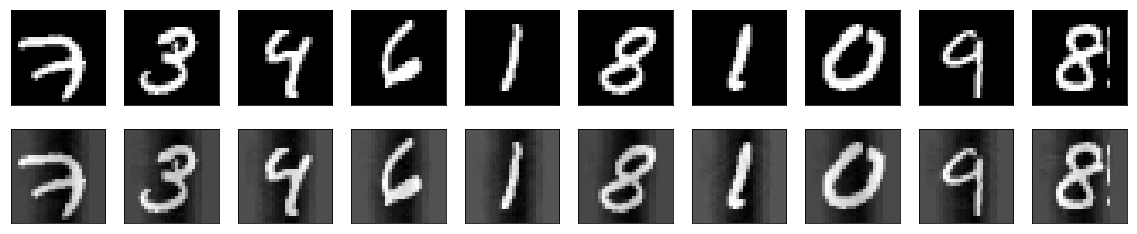
\includegraphics[scale=0.3]{CSC_reconstruction.png}
 % CSC_reconstruction.png: 1137x234 px, 72dpi, 40.12x8.26 cm, bb=0 0 1137 234
 \caption{Examples of reconstruction using CSC}
 \label{fig:CSC_recons}
\end{figure}

\begin{figure}[h]
 \centering
 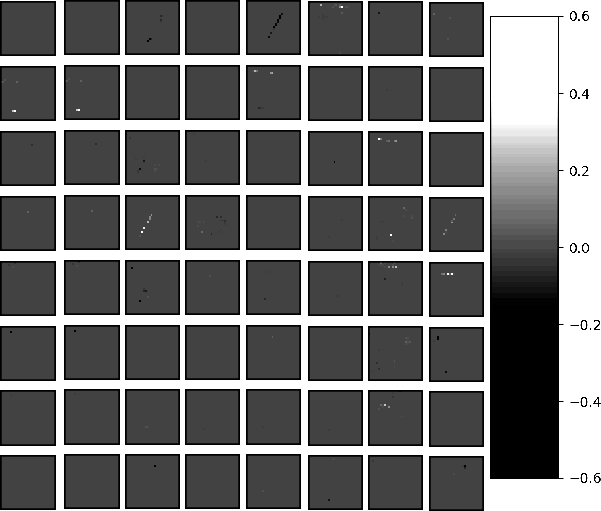
\includegraphics[scale=0.7]{MapActivation7.png}
 % MapActivation7.png: 601x511 px, 100dpi, 15.27x12.98 cm, bb=0 0 433 368
 \caption{Activation maps for a handwritten "7"}
 \label{fig:activationMaps}
\end{figure}

\begin{figure}[h]
 \centering
 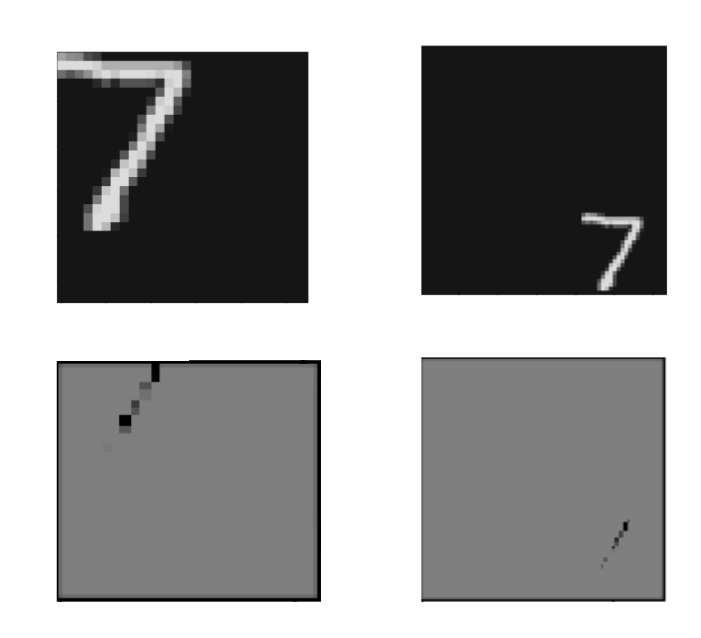
\includegraphics[scale=0.8]{CSC_Proof.png}
 % CSC_Proof.png: 701x638 px, 300dpi, 5.94x5.40 cm, bb=0 0 168 153
 \caption{Example of shift-invariance power in a characteristic features map ($5^{th}$ atom in the CSC dictionary)}
 \label{fig:CSCproof}
\end{figure}

As expected, Convolutional Sparse Coding detects the patterns in the input signal using the Sparse activation maps and the convolutional dictionary, which allows a good reconstruction(figure \ref{fig:CSC_recons}). But, as we can see in figure \ref{fig:activationMaps} and \ref{fig:CSCproof} in the activation maps, we obtained new patterns which are shift variant. Then we cannot apply the classification directly to these activation maps. To solve this problem, we tried different methods:
\begin{itemize}
 \item Max or Mean global pooling for each activation map:\\
 The objective was to create a unique activation card in which each pixel corresponds to the Max pooling of one of the 64 activation maps. But with these methods, we lose the pattern available in the activation maps, and consequently, discriminative pieces of information.
 \item Convolutional Sparse Coding on all activation maps:\\
 Apply on the activation maps a new convolutional sparse Coding. This method called Multi-Layer Convolutional Sparse Coding is described in the next chapter.
\end{itemize}
% 
% \newpage
% \subsection{Discussion}
% Using this examples we validate that CSC allow us to reconstruct our input data using filters, convolutions and activation maps. But we still cannot use activation maps for clustering or classification due to the non-discriminative reconstruction. Indeed, two seven in our test dataset haven't the same decomposition ( i.e. they don't have the same or close activation maps).

\newpage
\chapter{Discriminative Convolutional Sparse Coding}
% L'idée : Multi couche -> ML-CSC
% On rajoute un terme pour être sur que c'est discrimnant
\label{chap:SupervisedConv}
% \begin{figure}[h]
%  \centering
%  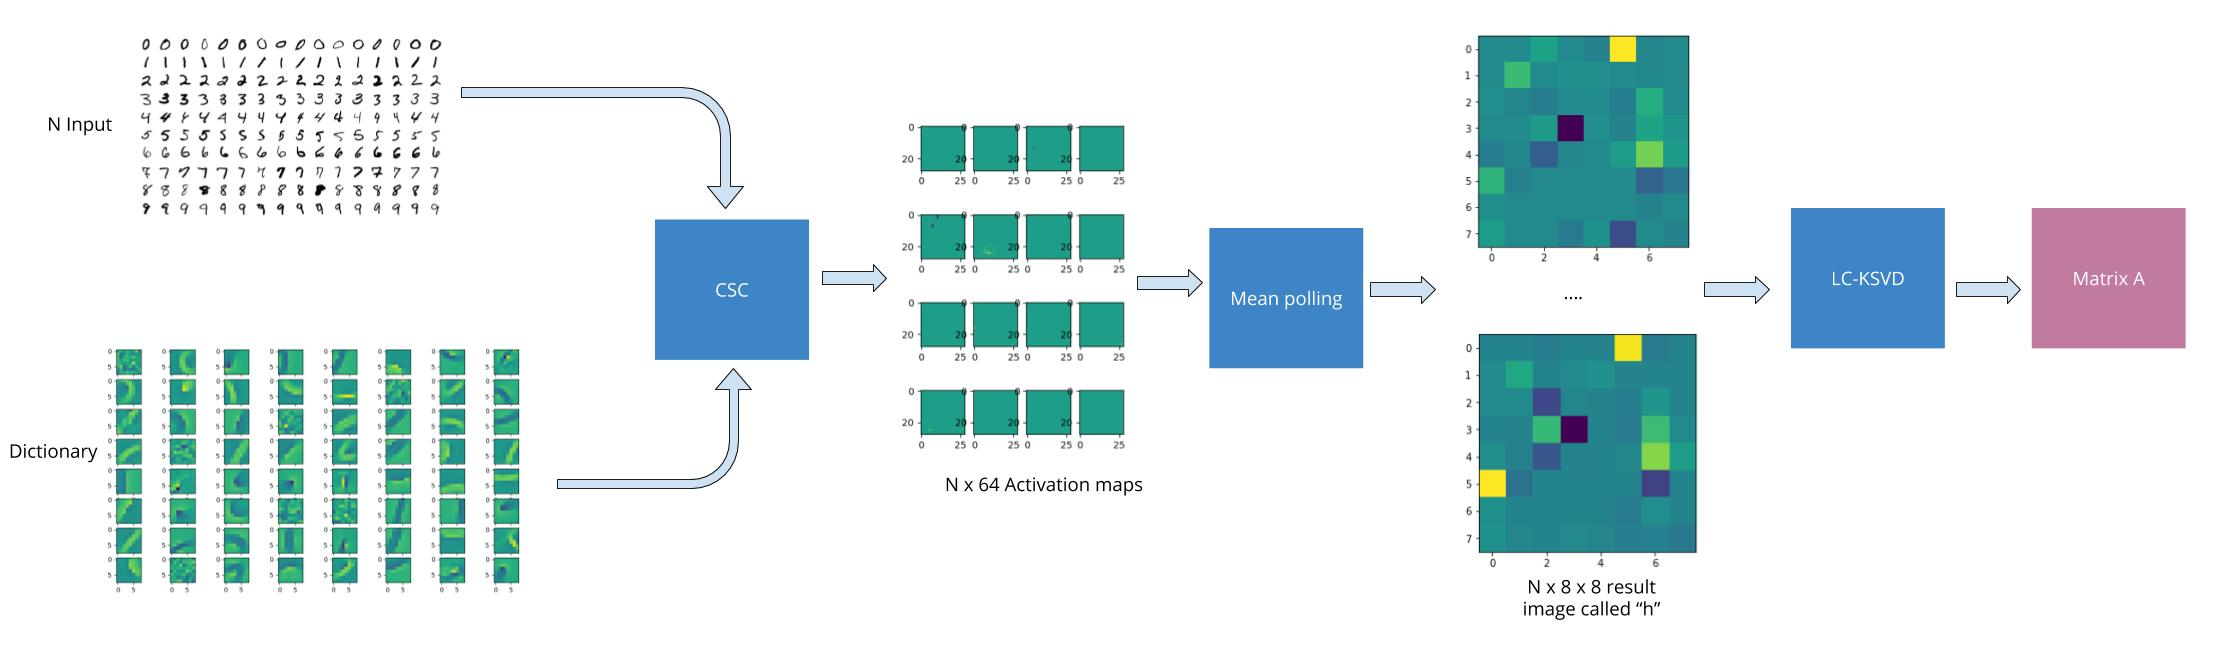
\includegraphics[scale=0.2]{Training_phase.jpg}
%  % Training phase.jpg: 2217x648 px, 72dpi, 78.21x22.86 cm, bb=0 0 2217 648
%  \caption{Training phase}
% \end{figure}
% \begin{figure}[h]
%  \centering
%  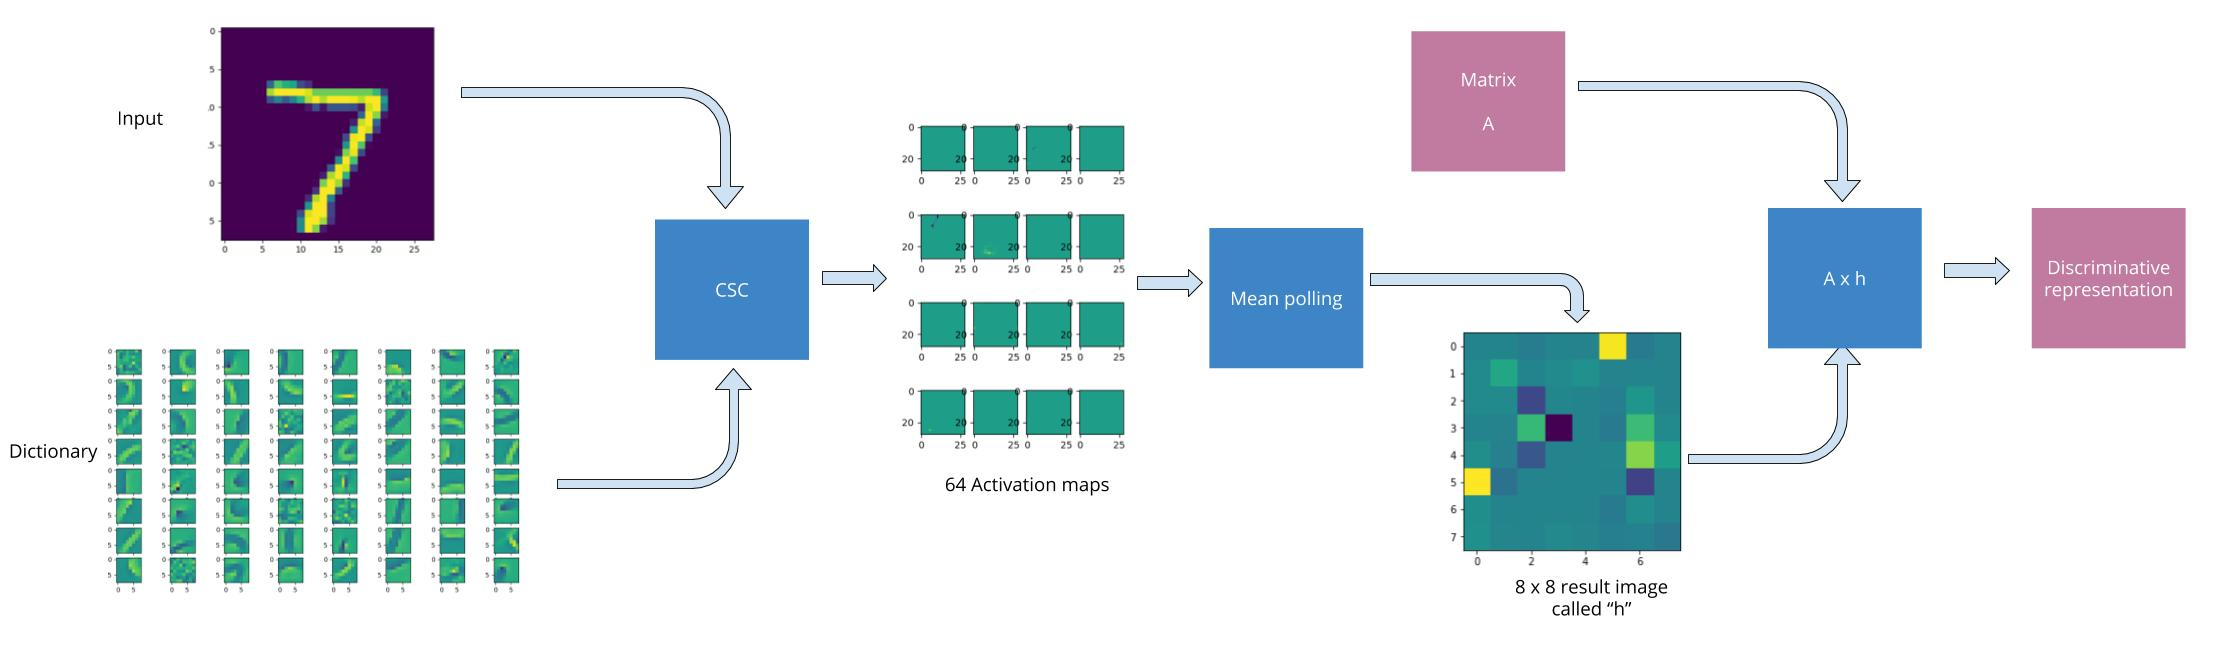
\includegraphics[scale=0.2]{Test_phase.jpg}
%  % Test phase.jpg: 2217x648 px, 72dpi, 78.21x22.86 cm, bb=0 0 2217 648
%  \caption{Test phase}
% \end{figure}
\section{ML-CSC}
In order to get a discriminative Convolutional Sparse Coding, \cite{DBLP:journals/corr/abs-1708-08705,8398588} proposed to extend the CSC model to a Multi-Layers version (called ML-CSC). Indeed,  adding a new CSC layer allows the algorithm to capture more complex patterns.\\
Add a new layer corresponds to get the features maps $Z$ obtained by CSC in the previous layers and use them like the input signal with a new dictionary, in other word $D_1$  (layer 1's dictionary) contain simple patterns, the convolution product $D_1 * D_2$ contains  a linear combination of atoms from $D_1$, merging them to create more complex patterns, called molecules. Mathematically,for $L$ layers:
\begin{center}
 $X = D_1 * Z_1$ \hspace{1cm} Layer 1\\
 $Z_1 = D_2 * Z_2$\hspace{1cm} Layer 2\\
 $Z_2 = D_3 * Z_3$\hspace{1cm} Layer 3\\
 \dots\\
 $Z_{L-1} = D_L * z_L$ \hspace{1cm} Layer L\\
 Then X can be rewriten by:\\
 $X = D_1 * D_2 * D_3 *\dots *D_L * z_L$
\end{center}
Then it is possible to rewrite the dictionary learning algorithm to extend it to a multi-layer version:\\
\begin{algorithm}
 \caption{Multi-Layer Convolutional Dictionary Learning}
 \begin{algorithmic}
  \REQUIRE Training sample $\{x_1, x_2, \dots, x_k \}$, initial convolutional dictionaries $\{D_1, D_2, \dots, D_L \}$, the number of iterations for gradient descent T
  \FOR{$k=1, \dots, k$}
        \STATE Sparse Coding: $z_L \leftarrow \underset{z_L}{\argmin} \|x_k - D_L z_L\|^2_2  + \lambda \|z_L\|_1$
        \STATE \textit{/* Update dictionaries*/}
        \FOR{$i = L, \dots, 1$}
            \FOR{$t = 1, \dots, T$}
                 \STATE $D_i \leftarrow \mathcal{H}[D_i - \alpha ((y_k -D_i Z_i)Z_i^T) ] $
            \ENDFOR
        \ENDFOR
        \FOR{$t = 1, \dots, T$}
            \STATE $D_1 \leftarrow D_i - \alpha ((y_k -D_iZ_1) Z_1^T)$
        \ENDFOR
  \ENDFOR
 \end{algorithmic}
\end{algorithm}\\
Note that $D_1$ is not updated with the others dictionaries $D_i$, this is because its imposed that the other dictionaries $D_i$ are sparse to be sure that the feature maps $Z_i$ are also sparse. This is possible by applying the hard-thresholding operation $\mathcal{H}$ on them.
\section{Tests details}
For all our experimentations on ML-CSC we used a matlab demo writen by 
Jeremias Sulam \footnote{\url{https://sites.google.com/view/jsulam/}} (writer of \cite{DBLP:journals/corr/abs-1708-08705,8398588}) that he provided us. We want to thank him for that.
\subsection{Application of ML-CSC on MNIST}
\begin{figure}[h]
 \centering
 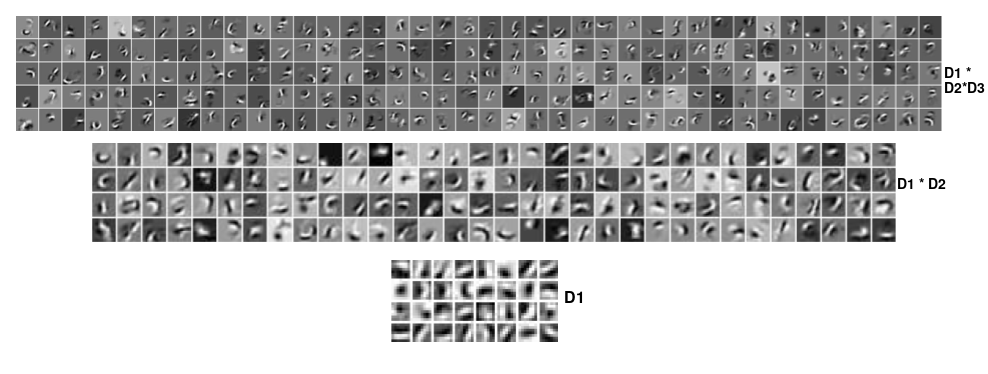
\includegraphics[scale=2]{Discriminative_CSC.png}
 % Discriminative CSC.png: 1001x266 px, 72dpi, 35.31x9.38 cm, bb=0 0 1001 266
 \caption{Dictionary's atoms at each layer}
 \label{fig:DCSC}
\end{figure}
\begin{figure}[h]
 \centering
 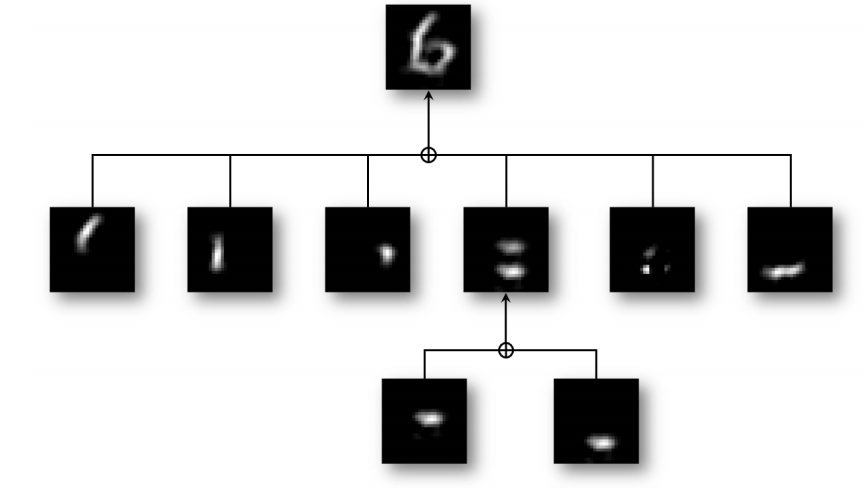
\includegraphics[scale=0.3]{decomp.png}
 % decomp.png: 864x488 px, 96dpi, 22.86x12.91 cm, bb=0 0 648 366
 \caption{From atoms to molecules: Illustration of the ML-CSC
model for a number 6. Two local convolutional atoms (bottom
row) are combined to create slightly more complex structures
– molecules – at the second level, which are then combined
to create the global atom representing, in this case, a digit \cite{DBLP:journals/corr/abs-1708-08705}}
 \label{fig:decomp}
\end{figure}

Here we see in figure \ref{fig:DCSC}the 3 layers of dictionaries with the learned forms. The deeper the dictionary got the more complex forms and therefore discriminative. In the figure \ref{fig:decomp} a reconstruction of a 6 is displayed. 

\subsection{Classification for ML-CSC}

With the Multi-layer Convolutional Sparse Coding, if we try to classify the obtained features we got:
\begin{itemize}
 \item SVM Accuracy = 93,67\%
 \item K-means Accuracy = 11,46\%
\end{itemize}
The problem here is that once again, we get bad results for K-means because the representations for the same classes can be different and the only way to solve it is to use the information of the labels that we have in the supervised setting. To address this problem we proposed a new method based on LC-KSVD.
\newpage
\section{LC-ML-CSC}
SAs we used Label-Consistent Sparse Coding instead of traditional Sparse Coding to get more discriminating Sparse coefficients, we want to create a new convolutional Multi-Layer Sparse Coding model that adds a consistent Label term: We called it \textit{Label Consistent Multi-Layer Convolutional Sparse coding} (LC-ML CSC).\\
We already explained what is the label consistent term and the multi-layers convolutional Sparse Coding, thus we can already present the LC-ML CSC algorithm:
\begin{algorithm}
\caption{Labels Consistent Multi Layers Convolutional Sparse Coding (LC-MLCSC )}
\begin{algorithmic} 
\REQUIRE Y: input data, Q: discriminative matrix
\FOR{$k = 1,\dots,K$} 
    \STATE $y_k \leftarrow $ The $k^{th}$ batch of Y
    \STATE \textit{/* Sparse Coding */} 
    \STATE $z_{kL} = \underset{z_k}{\argmin} \underset{CSC\ normal}{\underbrace{\|y_k - D^L z_k\|^2_2 +\alpha \|z_k\|_1}} + \underset{LC composant}{\underbrace{\beta \|Q -A z_k\|}}$ 
    \STATE $ = z_k  - \alpha(D^T (Dz_k -y_k) + \lambda(sign(z_k)) + \beta (A^T(A z_k -Q)))$
    \STATE \textit{/* Dictionary Update */}
    \FOR{$i=L, \dots, L $}
        \STATE $D_i \leftarrow \mathcal{H}[D_i - \alpha ((y_k -D_iz_k)z_k^T) ] $
    \ENDFOR
    \STATE \textit{/* Update Matrix A */}
    \STATE $A \leftarrow A + \alpha (\beta (Q-Az_k)z_k^T)$
\ENDFOR
\RETURN $z_k$, D, A
\end{algorithmic}
\end{algorithm}
% \begin{algorithm}
% \caption{Labels Consistant Multi Layers Convolutional Sparse Coding 2(LC-MLCSC 2)}
% \begin{algorithmic} 
% \REQUIRE Y, Q
% \FOR{$k = 1,\dots,K$} 
%     \STATE $y_k \leftarrow $ Le $k^{eime}$ batch de Y
%     \STATE Sparse Coding: 
% \STATE Sparse Coding: $z_L \leftarrow \underset{z_L}{\argmin} \|x_k - D_L z_L\|^2_2  + \lambda \|z_L\|_1$
%     \STATE Dictionary Update:
%     \FOR{$i=L, \dots, L $}
%         \STATE $D_i \leftarrow \mathcal{H}[D_i - \alpha ((y_k -D_iz_k)z_k^T) ] $
%     \ENDFOR
%     \STATE Mise à jour de la matrice A:
%     \STATE $A \leftarrow A + \alpha (\beta (Q-Az_k)z_k^T)$
% \ENDFOR
% \RETURN $z_k$, D, A
% \end{algorithmic}
% \end{algorithm}

However, at the moment when we write these internship report the LC-ML CSC still a work in progress method. And we don't have a good result in classifying even with SVM. That why we will not present the results of this method here.


%====================PART 2 SPARSE CODING FOR SR=========
\newpage
%\chapter{Sparse Coding for speech recognition}
%In this part of the paper we will see novel feature exraction technique based on the principles of sparse coding \cite{DL_speech_reco}. Sparse codigin deals with the problem of how represent a given audio input as a linear combination of a minimum number of basis function. The weights of the linear combination are used as feature for speech recognition (acoustic modeling). Note the input dimensionality is typically \textbf{much} less than the number of atoms in the dictionary \textit{i.e.} we use overcomplete dictionary.\\
%We use Sparse Coding algorithm as describe before and we get the dictionary D and  the matrix of sparse coefficients  h.\\
%\paragraph{Reflection path} In \cite{DL_speech_reco} they used spectro-temporal speech domain wich is obtained by performing a short time Fourier transform (STFT) with an analysis window of length 25 ms and a frameshit of 10 ms on t- Auto-encoder as a Deep learning approchhe input signal. Log critical band energies are subsequently obtained by projecting the magnitude square values of the STFT output on a set of frequency weights, which are equally spaced on the Bark frequence scale, and then applying a logarithm on the output projections.
%\newpage

\chapter{Auto-encoders}
\label{chap:AE}
\section{Principle}
The second feature extraction method we used during this internship was AutoEncoder \cite{Rumelhart:1986:LIR:104279.104293}. Autoencoder (AE) is an unsupervised neural network algorithm that takes a signal as input and tries to reconstruct the same signal as the output. Generally, AE is composed of three parts (see figure \ref{fig:AE} \footnote{We take the convention in the figure that all circles can be anything such as Conv2D + Pooling, Dense, \dots}):
\begin{itemize}
 \item Encoder 
 \item Latent Space Representation (Red box in figure \ref{fig:AE})
 \item Decoder
\end{itemize}
 
\begin{figure}[h]
 \centering
 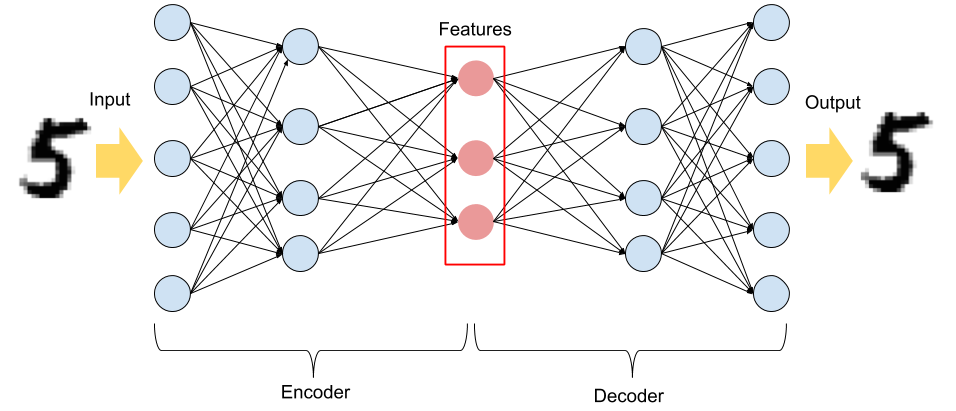
\includegraphics[scale=0.5]{AutoEncoder.png}
 % AutoEncoder.png: 956x411 px, 72dpi, 33.73x14.50 cm, bb=0 0 956 411
 \caption{Basic architecture of AutoEncoder}
 \label{fig:AE}
\end{figure}
Encoder and Decoder part work in the same way as a simple artificial neural network: a Feed Foward propagation algorithm to get the output from the input and Backward propagation of the error from the output to the input. The main difference with an artificial neural network is the Latent Space Representation which is typically a hidden layer located between the encoder and the decoder, with fewer neurons than any layers in Encoder or Decoder.\\
After the training, AutoEncoder can encode a certain set of data with less dimensionality than the input. It widely uses for feature extraction, segmentation, deconvolution, colorization, denoising,\dots\\
During the internship we tried two main architectures of AutoEncoder:
\begin{itemize}
 \item Sparse AutoEncoder, which has approximately the same behavior the Sparse Coding.
 \item Label Consistent AutoEncoder, which is a model we proposed based on the idea of Label-Consistent Sparse Coding.
\end{itemize}

\section{Sparse AutoEncoder}
In the respect of \textit{Sparseland} assumptions, \cite{DBLP:journals/corr/MakhzaniF13} introduced the K-Sparse AutoEncoder. The goal is the same as Sparse Coding, we want to compute a sparse representation from an input signal but the method is different. Here we do not have the dictionary directly, we have an Encoder that finds the sparse representation for us using artificial neurons or convolution blocks.\\
To allows the Autoencoder to find this sparse representation we must add a term in the loss function. It is called a regularizer, which is applied to the last layer of our encoder. We decided to keep using the $l_1$ norm for this regularizer.\\ 
Unlike the traditional Sparse Autoencoder, we decided to use more hidden units at the end of the encoder (cf figure \ref{fig:SAE}). With this addition, we create a discriminative representation instead of compressive representation.\\
\begin{figure}[h]
 \centering
 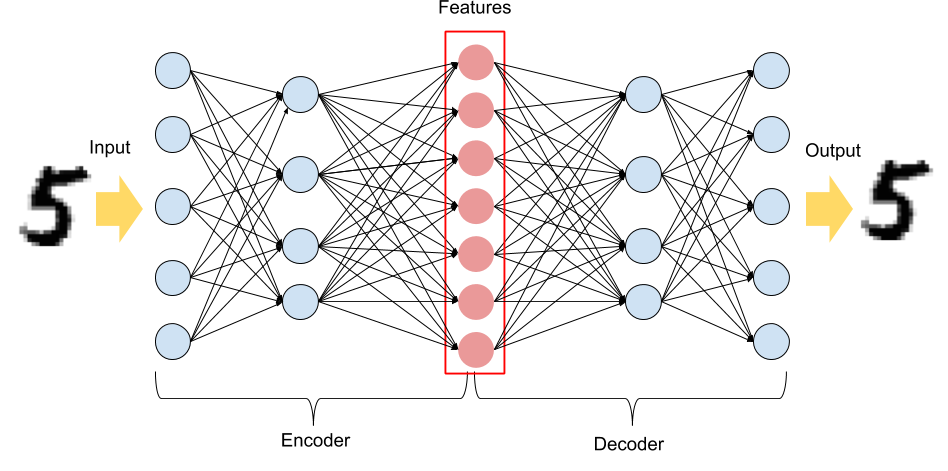
\includegraphics[scale=0.5]{sparse_AutoEncoder.png}
 % sparse AutoEncoder.png: 948x471 px, 72dpi, 33.44x16.62 cm, bb=0 0 948 471
 \caption{Example of Sparse AutoEncoder architecture}
 \label{fig:SAE}
\end{figure}

\newpage
\section{Labels Consistent AutoEncoder}
We proposed a new Autoencoder model for extraction of discriminative features. For this model, we were inspired by the Label-Consistent Sparse Coding and especially the Q matrix. Our idea is to bring the information on the label by encouraging the use of certain filters for a class.\\
However, we also want to keep the reconstruction. To achieve these two objectives, we decided to create two parallel branches, one for each problem (we show an example of our model architecture in figure \ref{fig:LC_AE}).\\
We called this model \textit{Label Consistent AutoEncoder}.  To fit with our previous studies  (especially CSC's method) we also use convolution blocks and pooling blocks for encoding, convolution and upsampling for decoding and dense block for the label consistent term.\\
We also tested this model with the Sparsity constraint to see if it would improve the results. We called this model \textit{Labels-Consistent Sparse Autoencoder}.\\
\begin{figure}[h]
 \centering
 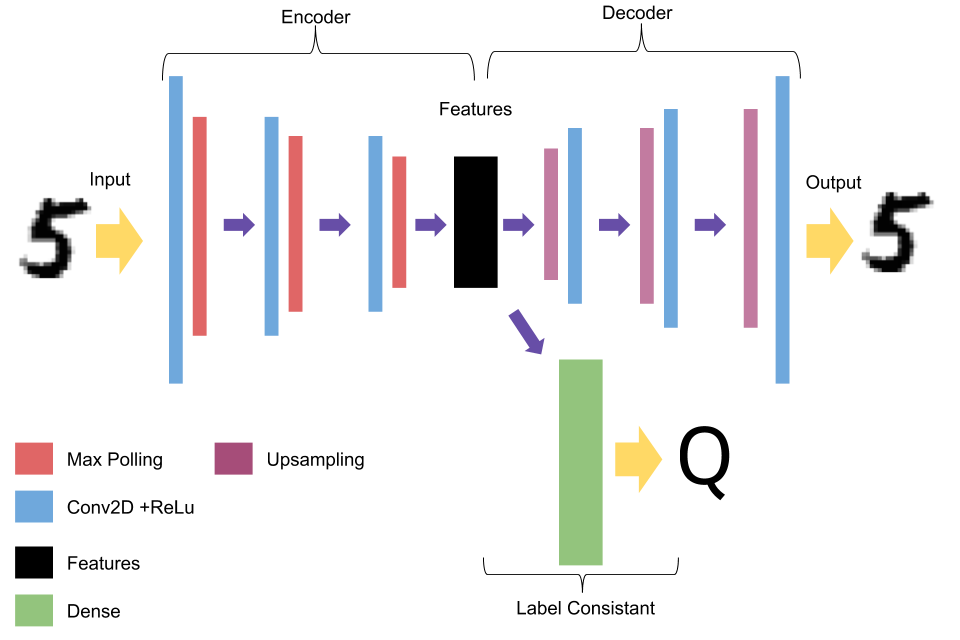
\includegraphics[scale=0.5]{LC_AutoEncoder.png}
 % LC_AutoEncoder.png: 964x627 px, 72dpi, 34.01x22.12 cm, bb=0 0 964 627
 \caption{Example of Label Consistant Autoencoder architecture}
 \label{fig:LC_AE}
\end{figure}
In addition, we train a A matrix in the same way as we did for $A_0$ in the LC-KSVD and multiply this A matrix with the features to get a more discriminative representation.
\newpage
\section{Experimentation details}
\subsection{Application of different Autoencoder on MNIST}
\subsubsection{K Sparse Autoencoder}
\begin{figure}[h]
 \centering
 \includegraphics[scale=0.4]{SAE.png}
 % SAE.png: 1130x230 px, 72dpi, 39.87x8.12 cm, bb=0 0 1130 230
 \caption{Reconstruction using decoder and encoded data}
 \label{fig:SAE_result}
\end{figure}

\begin{figure}[h]
 \centering
 \includegraphics[scale=0.4]{KSparseAE_CONV.png}
 % KSparseAE_CONV.png: 1099x231 px, 72dpi, 38.78x8.15 cm, bb=0 0 1099 231
 \caption{K Sparse Autoencoder using convolution, pooling, upsampling results}
 \label{fig:SAEconv}
\end{figure}
Here, we see that reconstruction is better in the context of convolution utilization (figure \ref{fig:SAEconv}) rather than with dense (figure \ref{fig:SAE}). This is explained by the fact that the method with Dense has only one layer whereas the method with convolution is deeper.
\subsubsection{Labels Consistent Autoencoder}
\begin{figure}[h]
 \centering
 \includegraphics[scale=0.3]{LCAE.png}
 % LCAE.png: 1490x812 px, 100dpi, 37.85x20.62 cm, bb=0 0 1073 585
 \caption{MNIST samples with the  LC-Autoencoder}
 \label{fig:LCAE}
\end{figure}
\subsubsection{Label Consistent Sparse Autoencoder}
\begin{figure}[h]
 \centering
 \includegraphics[scale=0.3]{Sparse-LCAE.png}
 % Sparse-LCAE.png: 1490x812 px, 100dpi, 37.85x20.62 cm, bb=0 0 1073 585
 \caption{MNIST samples with the Sparse LC-Autoencoder}
 \label{fig:SLCAE}
\end{figure}
In figure \ref{fig:LCAE} and figure \ref{fig:SLCAE} we can see that there is a good reconstruction but especially that the discriminating features $A*Features$ are perfect for classification, indeed, there is a white band at a precise location depending on the number label.
\subsection{Classification for Autoencoder}


\begin{center}
\begin{tabular}{|c|c|c|}\hline
× & \textbf{SVM accuracy} & \textbf{K-means accuracy}\\\hline
\textbf{K Sparse AE (Dense)} & 0.91 & 0.22\\\hline
\textbf{K Sparse AE (Conv with 32 filters)} & 0.96 & 0.19\\\hline
\textbf{K Sparse AE (Conv with 10 filters)} & 0.95 & 0.23\\\hline
\textbf{Label Consistent AE} & 0.98 & 0.98\\\hline
\textbf{LC Sparse AE} & 0.98 & 0.98\\\hline
\end{tabular}
\end{center}
It is clear that the results of the different autoencoders are good when using an SVM as a classifier. Nevertheless, the addition of the Label Consistency branch allows a clear improvement both on the SVM but also on the K-means, going to classification results of over 98\%. 

    %\input{ApplicationAE.tex}
\newpage
\chapter{Conclusion}
\label{chap:Conclusion}
As a reminder, all results of this internship are:\\

{%
\newcommand{\mc}[3]{\multicolumn{#1}{#2}{#3}}
\begin{center}
\begin{tabular}{lll}\cline{1-1}
\hline
\mc{3}{c}{Summary table of accuracy depending on the methods}\\\cline{1-3}
× & × & ×\\\hline
\mc{1}{|c|}{×} & \mc{1}{c|}{K-means Accuracy} & \mc{1}{c|}{SVM accuracy}\\\hline
\mc{1}{|c|}{Traditional Sparse Coding} & \mc{1}{c|}{0.13} & \mc{1}{c|}{0.90}\\\hline
\mc{1}{|c|}{LC-KSVD} & \mc{1}{c|}{0.78} & \mc{1}{c|}{0.91}\\\hline
\mc{1}{|c|}{ML-CSC} & \mc{1}{c|}{0.11} & \mc{1}{c|}{0.94}\\\hline
\mc{1}{|c|}{Sparse AE (Dense)} & \mc{1}{c|}{0.22} & \mc{1}{c|}{0.91}\\\hline
\mc{1}{|c|}{Sparse AE(Convolution)} & \mc{1}{c|}{0.19} & \mc{1}{c|}{0.96}\\\hline
\mc{1}{|c|}{LC-AutoEncoder} & \mc{1}{c|}{0.98} & \mc{1}{c|}{0.98}\\\hline
\mc{1}{|c|}{LC-Sparse AutoEncoder} & \mc{1}{c|}{0.98} & \mc{1}{c|}{0.98}\\\hline
\end{tabular}
\end{center}
}%

On the first hand, Statistical and deep learning methods for discriminant feature extraction is an important open problem that requires the introduction of new methods to enable the increasing of correct classification for many problems as Speech recognition. 
During this internship, we were able to compare different statistical methods based on the "Sparseland" hypothesis but also on the most recent deep learning methods.\\
 All results are relatively close with the SVM classifier (approximatively 90\%). However, only Label consistency term brings good result for the K-means classifier (approximatively 90\% for the Label Consistency versus 10\% for the others) because the information from the label is brought in during the trainning. \\
At the end of our research, we found that the LC-AutoEncoder and his sparse version allows good classification using both classifiers, SVM and K-means.\\

In general, adding label information with a label consistency constraint, or more generally directly with the label information improves the results of various methods (Sparse Coding, AutoEncoder, Sparse AutoEncoder) and we hope to get the same improvement for the Mutli-layer Convolutional Sparse Coding with the model Label-Consistent ML-CSC. It remains a job to be done, but we now know that there will already be at least two persons to take it back and improve our results.\\

On the other hand, this internship was an opportunity to discover in detail the world of research and all related challenges. The cross-disciplinary field between statistical approach and deep learning was very interesting, especially now, when the world is becoming more and more interested in deep learning. It is important for us to have the theoretical justifications of our models in order to be sure of the results they produce. This internship allowed us to obtain new skills, whether in optimization, machine learning (particularly deep learning) and signal processing.\\
It was also interesting to take part in the life of a laboratory during this internship, to discover other people's work, to offer our opinion to help and to share our personal experiences.

\bibliographystyle{plain}
\bibliography{efficient-sparse-coding-algorithms.bib}


\end{document}
